\documentclass{article}
\usepackage[margin=1.95cm]{geometry}

\usepackage{enumitem}
\setitemize{noitemsep,topsep=1pt,parsep=1pt,partopsep=1pt}
\usepackage[utf8]{inputenc}
\usepackage{amsmath,amsfonts,amsthm,amssymb}
\usepackage{xspace}
%\usepackage{algorithmic}
\usepackage{graphicx}
\usepackage{textcomp}
\usepackage{xcolor}
\usepackage{tikz,tkz-tab}
\usetikzlibrary{positioning,chains,fit,shapes,calc,arrows.meta,automata,arrows,decorations.markings,patterns}
\usepackage{tkz-graph}
\usepackage{tabularx}
\usepackage{subcaption}
\usepackage{placeins}  % Add this to your preamble

\usetikzlibrary{decorations.pathreplacing,calligraphy}
\usepackage{multirow}
\usepackage{hhline}
\usepackage{url}
%\usepackage{hyperref}
%\usepackage{paralist}
\usepackage{booktabs,makecell}
%\usepackage{todonotes}
\usepackage[ruled, linesnumbered]{algorithm2e}
\DontPrintSemicolon
\usepackage{xcolor}

\usepackage{etoolbox}
\def\tablename{Table}

\SetKwRepeat{Do}{do}{while}
\SetKw{Break}{break}
\SetKwFor{When}{when}{do}{end}

\DeclareMathOperator*{\argmin}{arg\,min}

\newtheorem{lemma}{Lemma}
\newtheorem{remark}{Remark}
\newtheorem{theorem}{Theorem}
\newtheorem{proposition}{Proposition}
\newtheorem{corollary}{Corollary}
\newtheorem{definition}{Definition}




%% Macros
\newcommand\fair{\textsc{Fair}\xspace}
\newcommand\ratio{R\xspace}
\newcommand\newrat{\textsc{newR}\xspace}
\newcommand\task{\mathcal{T}}
\newcommand\la{\ensuremath{\lambda}\xspace}
\newcommand\pp{\ensuremath{\mathbf{p}}\xspace}
\newcommand\pb{\ensuremath{\vec{p}}\xspace}
\newcommand\ppb{\ensuremath{\mathbf{p}}\xspace}
\newcommand\sstb{\ensuremath{\mathbf{s}}\xspace}
\newcommand\stb{\ensuremath{\vec{s}}\xspace}
\newcommand\one{\ensuremath{\mathbf{1}}\xspace}
\newcommand\ff{\ensuremath{\mathbf{f}}\xspace}
\newcommand\QQ{\ensuremath{\mathbf{Q}}\xspace}
\newcommand\st{\ensuremath{\mathbf{s}}\xspace}
\newcommand\alg{\textsc{alg}\xspace}
\newcommand\opt{\textnormal{opt}\xspace}
\newcommand\ftlist{\textsc{FT-List}\xspace}
\newcommand\listf{\textsc{List-F}\xspace}
\newcommand\listfshort{\textsc{LF}\xspace}
\newcommand\greedyRL{\textsc{Greedy-RL}\xspace}
\newcommand\ggreedy{\textsc{L-Increment}\xspace}
\newcommand\ggreedyfull{\textsc{Local-Increment}\xspace}
\newcommand\ggreedyshort{\textsc{LI}\xspace}
\newcommand\LBFF{$\textnormal{LB}_{\textnormal{ff}}$\xspace}
\newcommand\LBFW{$\textnormal{LB}_{\textnormal{fw}}$\xspace}
\newcommand\LBE{$\overline{\textnormal{LB}}$\xspace}

\newcommand\lpalist{\textsc{Lpa-List}\xspace}
\newcommand\set{\textsc{Set}\xspace}
\newcommand\ect{\textsc{Ect}\xspace}
\newcommand\lpa{\textsc{Lpa}\xspace}
\newcommand\listt{\textsc{List}\xspace}
\newcommand\batch{\textsc{Batch-List}\xspace}

\newcommand\ROO{\textsc{Roo}\xspace}
\newcommand\COM{\textsc{Com}\xspace}
\newcommand\AMD{\textsc{Amd}\xspace}
\newcommand\GEN{\textsc{Gen}\xspace}

\newcommand{\new}[1]{\textcolor{blue}{#1}}
\newcommand{\neww}[1]{\textcolor{blue}{#1}}
\newcommand{\nnew}[1]{\textcolor{blue}{#1}}
\usepackage[colorinlistoftodos,prependcaption,textsize=footnotesize]{todonotes}
\newcommand{\LP}[2][inline]{\todo[color=green!50,#1]{\sf \textbf{Lucas:} #2}
\xspace}
\newcommand{\HS}[2][inline]{\todo[color=red!50,#1]{\sf \textbf{Hongyang:} #2}
\xspace}

\newenvironment{proofsketch}{%
  \renewcommand{\proofname}{Proof sketch}\proof}{\endproof}
  
\begin{document}

\title{New results, Fair Heuristic}

\begin{abstract}
\LP{From TOPC paper}
The problem of scheduling moldable tasks on multiprocessor systems with the objective of minimizing the overall completion time (or makespan) has been widely studied, in particular
when tasks have dependencies (i.e., task graphs), or when tasks are released on-the-fly
(i.e., online). However, few studies have focused on both (i.e., online scheduling of moldable task graphs).
In this paper, we design a new online algorithm and derive constant competitive ratios for this problem under several common yet realistic
speedup models (i.e., roofline, communication, Amdahl, and a general combination).
We also prove, for each model, a lower bound on the competitiveness of our algorithm, which is very close to the constant competitive ratio.
Finally, we provide the first lower bound on the competitive ratio of any deterministic online algorithm for the arbitrary speedup model,
which is not constant but depends on the number of tasks in the longest path of the graph.
\end{abstract}


\maketitle

\section{Introduction}
\LP{From TOPC24 paper}
This work investigates the online scheduling of parallel task graphs on a set of identical processors, where each task in the graph is \emph{moldable}.
In the scheduling literature, a moldable task (or job) is a parallel task that can be executed on an arbitrary but fixed number of processors. The execution time of the task depends upon the number of processors used to execute it, which is chosen once and for all when the task starts its execution but cannot be modified later on during execution. This corresponds to a variable static resource allocation, as opposed to a fixed static allocation (\emph{rigid} tasks) and to a variable dynamic allocation (\emph{malleable} tasks)~\cite{Feitelson96}.

Moldable tasks offer a nice trade-off between rigid and and malleable tasks: they easily adapt to the number of available resources, contrarily to rigid tasks, while being easy to design and implement, contrarily to malleable tasks. This explains that many computational kernels in scientific libraries for numerical linear algebra and tensor computations are provided as moldable tasks that can be deployed on a wide range of processor numbers. We assume that the scheduling of each task is non-preemptive and without restarts~\cite{Feldmann98_DAG}, which is a highly desirable approach to avoid high overheads incurred by checkpointing partial results, context switching, and  task migration.

Because of the importance and wide availability of moldable tasks,
scheduling algorithms for such tasks have received considerable attention. The scheduling problem comes in many flavors:

\begin{itemize}[leftmargin=*]
\item \textbf{Offline Scheduling vs. Online Scheduling.} In the offline version of the scheduling problem, all tasks are known in advance, before the execution starts. The problem is $\mathcal{NP}$-complete, and the goal is to design good approximation algorithms. On the contrary, in the online version of the problem,
tasks are released on the fly, and the objective is to derive competitive ratios~\cite{Sleator1985} for the performance of a scheduling algorithm
against an optimal offline scheduler, which knows in advance all the tasks and and their dependencies in the graph. The competitive ratio is established against all possible strategies devised by an adversary trying to force the online algorithm to take \emph{bad} decisions.
\item \textbf{Independent Tasks vs. Task Graphs.} There are two versions of the online problem, with independent tasks
or with task graphs.
For the version with independent tasks, the tasks are released on the fly and the scheduler discovers their characteristics only upon release. For the version with task graphs, the whole graph is released at the start, but the scheduler discovers a new task and its characteristics only when all of its predecessors have completed execution. In other words, the shape of the graph and the nature of the tasks are not known in advance and are revealed only as the execution progresses.
\end{itemize}

In this work, we investigate the most difficult instance of the problem, namely, the online scheduling of moldable tasks graphs, with the goal of minimizing the overall completion time, or the makespan.
Our main contribution resides in the design of a new online algorithm and in several new competitive ratios,
which greatly depend upon the speedup model of the tasks. Several common yet realistic speedup models have been introduced
and analyzed, including the roofline model, the communication model, the Amdahl's model, a general combination of them (see Section~\ref{sec.model} for definitions), \new{and an extension on the communication model}.
We provide a constant competitive ratio for each of these five models. 

\LP{To fill : In previous papers, we needed an exact model on the speedup model. Here we don't need anything and match or surpass previous algorithms, in competitive ratio and in performance in practice}



The rest of this paper is organized as follows. Section~\ref{sec.related} surveys related work.
The formal model and problem statement are presented in Section~\ref{sec.pb}.
Section~\ref{sec.alg} is the heart of the paper: we introduce a new online algorithm and prove its competitive ratios for different speedup models; we also prove a lower bound for each model.
Section~\ref{sec.lower} is devoted to proving a lower bound of any deterministic online algorithm for the arbitrary speedup model.
Finally, Section~\ref{sec.conclusion} concludes the paper and suggests future directions.

\section{Related Work}
\label{sec.related}
\LP{From TOPC paper}

Several prior studies have considered offline scheduling of independent moldable tasks,
and derived approximation results. While some results depend on specific speedup models
for the tasks, other results hold for the arbitrary model.
Turek et al.~\cite{Turek92} designed
a 2-approximation list-based algorithm for the arbitrary model. Furthermore, when each task only admits
a subset of all possible processor allocations, Jansen \cite{Jansen12_3over2} presented a $(1.5+\epsilon)$-approximation algorithm, which is tight since it was also shown that the problem cannot have an approximation ratio better than 1.5
unless $\mathcal{P} = \mathcal{NP}$~\cite{Johannes06_list}. For the monotonic model, where the execution
time is non-increasing and the area (processor allocation times execution time) is non-decreasing with the
number of processors, Jansen and Land~\cite{Jansen18_PTAS} further proposed a polynomial-time approximation scheme (PTAS).

For online scheduling of independent moldable tasks that are released on-the-fly, Ye et al.~\cite{Ye18_online} designed a 16.74-competitive algorithm.
They also explained how to transform an algorithm for rigid tasks whose makespan is at most $\rho$ times
the lower bound into a $4\rho$-competitive algorithm for moldable tasks. Further, some algorithms designed in the
offline setting will also work online if they make scheduling decisions independently for each task; see for
instance~\cite{Havill08_SET, Dutton07_ECT, Kell15_Improved}, which studied the communication model.

For offline scheduling of moldable tasks with dependencies,
Wang and Cheng~\cite{Wang92_DAG} showed that the earliest completion time algorithm is a $(3-2/P)$-approximation for the roofline model, where $P$ denotes the total number of processors on the platform.
For the monotonic model, Lep\`{e}re et al. \cite{Lepere01_DAG} proposed an algorithm with approximation ratio $3+\sqrt{5}$, which was later improved to 4.73 by Jansen and Zhang~\cite{Jansen06_DAG}.
Chen and Chu~\cite{Chen13_concave} further proposed improved approximations for a more restrictive model, where the area is a concave function and the execution time is strictly decreasing with the number of processors.

Feldmann et al.~\cite{Feldmann98_DAG} designed an online algorithm for
moldable tasks
with dependencies, under the roofline model.
By keeping the system utilization
above a given bound and by carefully tuning this bound, their algorithm
achieves 2.618-competitiveness, even when the task execution times and the DAG structure are unknown.
Canon et al.~\cite{Canon20_online} focused on hybrid platforms with several types of processors
(for instance, CPUs and GPUs), and derived competitive ratios depending on the number
of such resources, but they did not consider moldable tasks.

Benoit et al.~\cite{Benoit20_cluster, Benoit21_ieeetc} recently investigated the problem of scheduling independent moldable tasks subject to failures,
where tasks need to be re-executed after a failure until a successful completion.
This corresponds to a semi-online setting, since all tasks are known at the beginning, but
failed tasks are only discovered on-the-fly.
We do not consider task failures in this paper, but rather focus on the general
online scheduling of moldable task graphs (as in~\cite{Feldmann98_DAG}). However, our results can readily carry over to the failure scenario.

Table \ref{tab.references} summarizes the instances of different scheduling problems and the related papers under each instance.

\begin{table}[t]
\centering
\caption{Instances of the scheduling problem.}
\label{tab.references}
\begin{tabular}{|c|c|c|}
\hline
Problem Instance & Offline & Online\\ \hline
Independent moldable tasks & \cite{Turek92,Jansen12_3over2,Jansen18_PTAS}& \cite{Ye18_online, Havill08_SET, Dutton07_ECT, Kell15_Improved}\\ \hline
Moldable task graphs & \cite{Wang92_DAG,Chen13_concave, Lepere01_DAG, Jansen06_DAG} & \cite{Feldmann98_DAG}, [This paper] \\ \hline
\end{tabular}
\end{table}

\section{Problem Statement}
\label{sec.pb}
\LP{From TOPC Paper}
In this section, we formally present the online scheduling model and the objective function. We also show a simple lower bound on the optimal makespan, against which the performance of our online algorithms will be measured.

\subsection{Model and Objective}
\label{sec.model}

We consider the online scheduling of a \textbf{\emph{Directed Acyclic Graph (DAG)}} of moldable tasks on a platform with $P$ identical processors. Let $G = (V, E)$ denote the task graph, where $V = \{1, 2, \dots, n\}$ represents a set of $n$ tasks and $E \subseteq V \times V$ represents a set of precedence constraints (or dependencies) among the tasks. An edge $(i, j) \in E$ indicates that task $j$ depends on task~$i$, and therefore it cannot be executed before task~$i$ is completed. Task~$i$ is called the \textbf{\emph{predecessor}} of task~$j$, and task~$j$ is called the \textbf{\emph{successor}} of task~$i$. In this work, we do not consider the costs associated with the data transfers between dependent tasks.

The tasks are assumed to be \textbf{\emph{moldable}}, meaning that the number of processors allocated to a task can be determined by the scheduling algorithm at launch time, but once the task has started executing, its processor allocation cannot be changed. The execution time $t_j(p_j)$ of a task $j$ is a function of the number $p_j$ of processors allocated to it, and we assume that the processor allocation must be an integer between $1$ and $P$. In this paper, we focus on the following execution time functions:
\begin{itemize}
\item \emph{\textbf{Roofline Model}} \cite{Williams2009}:
\begin{align}
\label{eq.model.roof}
t_j(p_j) = \frac{w_j}{\min(p_j, \bar{p}_j)} \ .
\end{align}
This model assumes that the task has a linear speedup until a maximum degree of parallelism $\bar{p}_j \le P$.
\item \emph{\textbf{Communication Model}} \cite{Havill08_SET}:
\begin{align}
\label{eq.model.comm}
t_j(p_j) = \frac{w_j}{p_j} + c_j (p_j - 1) \ .
\end{align}
This model assumes that the work of the task can be perfectly parallelized, but there is a communication overhead when more than one processor is allocated, which increases linearly with the number of allocated processors.


\item \emph{\textbf{Amdahl's Model}} \cite{Amdahl67}:
\begin{align}
\label{eq.model.amdahl}
t_j(p_j) = \frac{w_j}{p_j} + d_j \ .
\end{align}
This model assumes that the task has a perfectly parallelizable fraction with work $w_j$ and an inherently sequential fraction with work $d_j$.


\item \new{\emph{\textbf{Power Communication Model}}
\begin{align}
\label{eq.model.powcomm}
t_j(p_j) = \frac{w_j}{p_j} + c_j (p_j)^{\gamma_j} \ .
\end{align}
Contrarily to the communication model where the communication cost grow linearly with the number of processor, we add an exponent $0 \leq \gamma_j \leq 1$ to address more possible scenarios. If $\gamma_j=0$ it corresponds to Amdahl's model whereas if $\gamma_j=1$, the communication cost grows linearly with $p_j$ as in the Communication Model.}

\item \emph{\textbf{General Model}}:
\begin{align}
\label{eq.exec_time}
t_j(p_j) = \frac{w_j}{\min(p_j, \bar{p}_j)} + d_j + c_j (p_j - 1) \ ,
\end{align}
\new{This model is a generalization of the last three models.}
\end{itemize}

From the execution time function of the task $j$, we can further define the \textbf{\emph{area}} of the task as a function
of the processor allocation as follows: $a_j(p_j) = p_j t_j(p_j)$. Intuitively, the area represents
the total amount of processor resources utilized over the entire period of task execution.

In this work, we consider the \textbf{\emph{online scheduling}} model, where a task becomes available
only when all of its predecessors have been completed. This represents a common scheduling model
for \textbf{\emph{dynamic task graphs}}, whose dependencies are only revealed upon task completions \cite{JOHNSON96_dynamic,Feldmann98_DAG,Agrawal10_dynamic,Canon20_online}.  Furthermore, when a task $j$ is available,
all of its execution time parameters (i.e., $w_j$, $\bar{p}_j$, $d_j$, $c_j$) become known
to the scheduling algorithm as well. The goal is to find a feasible schedule of the task graph that minimizes its overall completion time or \textbf{\emph{makespan}}, denoted by $T$. The performance of an online scheduling algorithm is measured by its competitive ratio: the algorithm is said to be \textbf{\emph{$c$-competitive}} if, for any task graph, its makespan~$T$ is at most $c$ times the makespan $T^{\opt}$ produced by an optimal offline scheduler, i.e., $\frac{T}{T^{\opt}} \le c$. Note that the optimal offline scheduler knows in advance all the tasks and their speedup models, as well as all dependencies in the graph. The competitive ratio is established against all possible strategies by an adversary trying to force the online algorithm to take bad decisions.

\subsection{Lower Bound on Optimal Makespan}

Given the execution time function in Equation (\ref{eq.exec_time}), let us define $s_j = \sqrt{w_j/c_j}$. We can then compute the maximum number of processors that should be allocated to the task as:
\begin{align}\label{eq.pjmax}
p_j^{\max} = \min\left(P, \bar{p}_j, \tilde{p}_j\right) \ ,
\end{align}
where\\[-.6cm]
\begin{align*}
\tilde{p}_j = \left\{\begin{array}{ll}
\lfloor s_j \rfloor, & \text{if } t_j(\lfloor s_j \rfloor) \le t_j(\lceil s_j \rceil)  \\
\lceil s_j \rceil, & \text{otherwise}
\end{array}\right .
\end{align*}
Indeed, allocating more than $p_j^{\max}$ processors to the task will no longer decrease its execution time while only increasing its area. Thus, we can safely assume that the processor allocation of the task should never exceed $p_j^{\max}$ by any reasonable algorithm.

Furthermore,  the task is said to satisfy the \textbf{\emph{monotonic}} property~\cite{Lepere01_DAG} if the following two conditions hold:
\begin{itemize}
\item The execution time is a \textbf{\emph{non-increasing}} function of the processor allocation, i.e., $t_j(p) \ge t_j(q)$ for all $1 \le p < q \le p_j^{\max}$; \LP{This assumption is unnecessary except for the minor dichotomic search in Algorithm~\ref{alg.allocate1}}
\item The area is a \textbf{\emph{non-decreasing}} function of the processor allocation, i.e., $a_j(p) \le a_j(q)$ for all $1 \le p < q \le p_j^{\max}$.
\end{itemize}

Note that the second condition above also suggests that the task cannot achieve superlinear speedup, i.e.,
\begin{align}\label{eq.speedup_bound}
\frac{t_j(p)}{t_j(q)} \le \frac{q}{p} \text{ for all } 1 \le p < q \le p_j^{\max} \ .
\end{align}

\begin{lemma}\label{lem.monotonic}
A task $j$ with execution time function given in Equation~\eqref{eq.exec_time} is monotonic if its processor allocation is in the range $[1, p_j^{\max}]$.
\end{lemma}
\vspace{-.2cm}
\begin{proof}
When the processor allocation is in the range $[1, p_j^{\max}]$, we have $p_j \le p_j^{\max} \le \bar{p}_j$. Thus, the execution time function simplifies to $t_j(p_j) = \frac{w_j}{p_j} + d_j + c_j (p_j - 1)$.
%\begin{align*}
%t_j(p_j) = \frac{w_j}{p_j} + d_j + c_j (p_j - 1) \ .
%\end{align*}
This is a convex function whose minimum value is achieved at $\tilde{p}_j$. Since we also have $p_j \le p_j^{\max} \le \tilde{p}_j$, it shows that the execution time is a non-increasing function of $p_j$ in the range $[1, p_j^{\max}]$.

Similarly, when $p_j \le p_j^{\max} \le \bar{p}_j$, the area becomes $a_j(p_j) =  p_j t_j(p_j) = w_j + d_jp_j + c_j(p_j^2 - p_j)$,
%\begin{align*}
%a_j(p_j) =  p_j \times t_j(p_j) = w_j + d_jp_j + c_j(p_j^2 - p_j) \ ,
%\end{align*}
which is non-decreasing for any $p_j \ge 1$.
\end{proof}

Based on Lemma \ref{lem.monotonic}, the minimum execution time of the task is achieved as $t_j^{\min} = t_j(p_j^{\max})$ and the minimum area of the task is achieved as $a_j^{\min} = a_j(1)$.
Further, we let $t_j^{\opt}$ and $a_j^{\opt}$ denote the execution time and area of the task under the processor allocation of an optimal schedule.
We now define two quantities that can be used as a lower bound of the optimal makespan.

\begin{definition}
Given the processor allocations of all the tasks in an optimal schedule,
\begin{itemize}
  \item the \textbf{\emph{total area}} $A^{\opt}$ of the task graph is the sum of the areas of all the tasks in the graph, i.e., $A^{\opt} = \sum_{j=1}^{n} a_j^{\opt}$.
  \item the length $L^{\opt}(f)$ of a path\footnote{A path $f$ consists of a sequence of tasks with linear dependency, i.e., $f = (j_{\pi(1)}, j_{\pi(2)}, \dots, j_{\pi(v)})$, where the first task~$j_{\pi(1)}$ in the sequence has no predecessor in the graph, the last task $j_{\pi(v)}$ has no successor, and, for each $2\le i\le v$, task $j_{\pi(i)}$ is a successor of task~$j_{\pi(i-1)}$.} $f$ in the graph is the sum of the execution times of all the tasks along that path, i.e., $L^{\opt}(f) = \sum_{j\in f}t_j^{\opt}$. The \textbf{\emph{critical path length}} $C^{\opt}$ of the graph is the longest length of any path in the graph, i.e., $C^{\opt} = \max_{f} L^{\opt}(f)$.
\end{itemize}
\end{definition}

Clearly, the optimal makespan cannot be smaller than $\frac{A^{\opt}}{P}$ and $C^{\opt}$. This follows from the well-known area and critical-path bounds for scheduling any task graph \cite{Graham69}.
% The minimum choice for both quantities ensures that they can serve as the lower bounds on the optimal makespan.
The following lemma states this result.
\begin{lemma}\label{lem.lower}
$T^{\opt} \ge \max \left(\frac{A^{\opt}}{P}, C^{\opt} \right)$.
\end{lemma}


\section{Online Algorithm}
\label{sec.alg}
\LP{Updated from TOPC Paper}
In this section, we present \new{\fair}, an online scheduling algorithm, and derive its competitive ratio for the general speedup model (Equation~(\ref{eq.exec_time})) and its three special cases. We also prove lower bounds on the competitiveness of our algorithm under these speedup models.

\subsection{Algorithm Description}

{
\begin{algorithm}[t]
    \footnotesize
	\caption{Allocate\_Processor($j,\ratio$)}\label{alg.allocate1}
    \KwIn{\neww{Task $j$ and Ratio $\ratio$ }}
    \KwOut{\neww{Processor allocation $p'_j$ for the task}}
    \tcp{Step 1: Initial Allocation}
    Compute $p_j^{\max}$ based on Equation (\ref{eq.pjmax})\;
    Compute $t_j^{\min} = t_j(p_j^{\max})$ and $a_j^{\min} = a_j(1)$\;
    Find an allocation $p_j \in [1, p_j^{\max}]$ that \new{minimizes $\ratio_j \triangleq \max_p\left(\frac{t_j(p)}{t_j^{\min}}, \frac{a_j(p)}{a_j^{\min}}\right)$}\;
    \tcp{Step 2: Allocation Adjustment}
    \lIf{$p_j > \lceil \new{\mu(R)} P \rceil$}
    {
        $p'_j \leftarrow \lceil \new{\mu(R)} P \rceil$ \textbf{else} $p'_j \leftarrow p_j$
    }
   \new{\Return $\ratio_j$\;}
\end{algorithm}
}

\new{We first introduce \fair's subroutine, Allocate\_Processor($j,\ratio$), that affects a number of processor to each task $j$ and is presented in Algorithm \ref{alg.allocate1}.}

It consists of two steps. The first step performs an initial allocation for the task, which is inspired by the \textbf{\emph{local processor allocation}} strategy proposed in \cite{Benoit20_cluster, Benoit21_ieeetc}. Specifically, for each possible allocation $p\in [1, p_j^{\max}]$, we define $g_j(p) \triangleq a_j(p)/a_j^{\min}$ to be the ratio between the area of the task and its minimum area, and $f_j(p) \triangleq t_j(p)/t_j^{\min}$ to be the ratio between the execution time of the task and its minimum execution time. We then find an allocation $p$ that minimizes \new{$\max_p(f_j(p),g_j(p))$. We denote as $\ratio_j$ this resulting maximum.} Since $g_j(p)$ is non-decreasing with $p$ and $f_j(p)$ is non-increasing with $p$, the above optimization problem can be efficiently solved using binary search in $O(\log P)$ time.


In the second step, the algorithm reduces the initial allocation to $\lceil \new{\mu(\ratio)} P \rceil$ if it is more than $\lceil \new{\mu(\ratio)} P \rceil$; otherwise the allocation will be unchanged. \new{It uses $\ratio$ which corresponds to the highest ratio we've seen so far among all the tasks that arrived in the system. More precisely, }

\begin{align}\label{eq.muR}
\new{\mu(\ratio)=\frac{2\ratio+1-\sqrt{4\ratio^2+1}}{2\ratio}}
\end{align}  

Let $p_j$ denote the initial allocation for the task and $p'_j$ the final allocation. Thus, after the second step, we have:
\begin{align}\label{eq.adjust}
p'_j = \begin{cases}
\lceil \new{\mu(\ratio)} P \rceil,  & \text{~if~} {p}_j > \lceil\new{ \mu(\ratio)} P \rceil \\
{p}_j, & \text{~otherwise~}
\end{cases} \ .
\end{align}
This step adopts the technique first proposed in \cite{Lepere01_DAG} and subsequently used in \cite{Jansen06_DAG, Jansen05_concave}.{\color{brown} The purpose is to enable the execution of more tasks at any time, thus potentially increasing the overall resource utilization of the platform and reducing the makespan.} \new{Finally, Algorithm~\ref{alg.allocate1} returns the ratio $\ratio$ obtained in the first step. }
\LP{I probably disagree or at least don't love the formulation, it's to avoid having some tasks ready and a poor processor utilization at the same time, which would not be efficient for the area nor the critical path and could be an issue in the worst case scenario}



Algorithm~\ref{alg.online} presents the pseudocode of the online scheduling algorithm, which at any time maintains the set of available tasks in a waiting queue $Q$. At time 0 or whenever a running task completes execution, it checks if new tasks have become available. If so, for each newly available task $j$, it finds a processor allocation $p_j$ for the task (using Algorithm \ref{alg.allocate1}) before inserting it into the queue $Q$. \new{Then, it checks whether any of the new task resulted in a higher ratio $\newrat$ than the one we had until then. If so, it updates the highest ratio $\ratio$ and update the processor allocation of all tasks in the waiting queue $Q$ (note that since $\mu(\ratio)$ decreases with $\ratio$, the allocation may only decrease). Finally}, it applies the well-known \textbf{\emph{list scheduling}} strategy \cite{Graham69} by scanning through all the available tasks in $Q$ and executing each one right away if there are enough processors. Note that tasks are inserted into the queue without any priority considerations, although in practice certain priority rules may work better.




{%\LinesNumberedHidden
\begin{algorithm}[t]
    \footnotesize
	\caption{\new{\fair}}
	\label{alg.online}
        initialize a waiting queue $Q$\;
        \new{$\ratio=1$\; } 
        \When{\textnormal{at time $0$ or a running task completes execution}}{
            \tcp{Processor Allocation}
            \new{$\newrat=\ratio$\;}
            \For{\textnormal{each new task $j$ that becomes available}}{
                \new{$\newrat=max(\newrat,$Allocate\_Processor($j,\ratio$))\;}
                insert task $j$ into the waiting queue $Q$\;
            }
            \new{\tcp{If the highest ratio changed, update processor allocation}
            \If{$\newrat > \ratio$}{
  			  $\ratio = \newrat$\;
 			   \For{\textnormal{each task $j$ in the waiting queue $Q$}}{
 		       Allocate\_Processor($j,\ratio$)\;
  			  }
			}		}
            \tcp{List Scheduling}
            \For{\textnormal{each task $j$ in the waiting queue $Q$}}{
                \If{\textnormal{there are enough processors to execute the task}}{
                    execute task $j$ now\;
                }
            }
		}
\end{algorithm}
}

\subsection{General Analysis Framework}\label{sec.framework}

We first outline a general analysis framework, under which the competitive ratio of the proposed online algorithm will be derived for different speedup models.
The framework is inspired by the analysis shown in \cite{Lepere01_DAG, Jansen06_DAG, Jansen05_concave} for list scheduling as well as the analysis used in \cite{Benoit20_cluster, Benoit21_ieeetc} for local processor allocation. Together, the result nicely connects the makespan of the online algorithm to the lower bound (Lemma \ref{lem.lower}), thus proving the competitive ratio.


\new{We start with a small lemma on the function $\mu(x)$ defined in Equation~\ref{eq.muR}}
\begin{lemma}
\label{lem.muprop}
\new{$\mu(x)=\frac{2x+1-\sqrt{4x^2+1}}{2x}$ is well defined, positive and decreasing in $[1, \infty)$. Furthermore, $\mu(x) \leq \frac{3-\sqrt{5}}{2}$ and $\frac{x}{1-\mu(x)}=\frac{1}{\mu(x)}-x$ increases with $x$.}
\end{lemma}
\begin{proof}
\new{For $x\geq 1$, $\mu(x)$ has the same sign as $2x+1-\sqrt{4x^2+1} > 2x+1-\sqrt{4x^2+4x+1}=0$, hence it is well defined and positive. To show the other results, we first define $v(x)=\frac{x}{1-\mu(x)}$
\begin{align*}
v(x)&=\frac{x}{1-\mu(x)}=\frac{x}{\frac{\sqrt{4x^2+1}-1}{2x}}= \frac{2x^2}{\sqrt{4x^2+1}-1}=\frac{\sqrt{4x^2+1}+1}{2}\\
&= \frac{2x+1+\sqrt{4x^2+1}}{2}-x=\frac{(2x+1+\sqrt{4x^2+1})(2x+1+\sqrt{4x^2-1})}{2(2x+1-\sqrt{4x^2+1})}-x \\
&= \frac{(2x+1)^2-(4x^2+1)}{2(2x+1-\sqrt{4x^2+1})}-x =\frac{1}{\mu(x)}-x
\end{align*}
With $v(x)= \frac{\sqrt{4x^2+1}+1}{2}$, we have shown $v(x)$ is increasing, and with $v(x)=\frac{1}{\mu(x)}-x$, we have shown $\frac{1}{\mu(x)}$ must increase since $v(x)$ increases and $-x$ decreaes with $x$.}
\end{proof}

Recall that $T$ denotes the makespan of the online scheduling algorithm. Since the algorithm allocates and de-allocates processors upon task completions, the schedule can be divided into a set $\mathcal{I} = \{I_1, I_2, \dots\}$ of non-overlapping intervals, where tasks only start (or complete) at the beginning (or end) of an interval, and the number of utilized processors does not change during an interval. \new{Since no tasks gets ready within an interval, the current value of $\ratio$ is also constant and denoted as $\ratio(I)$ for each interval  $I \in \mathcal{I}$. For simplicity we define as $\mu_I$ as $\mu(\ratio(I))$. Finally, }let $p(I)$ denote its processor utilization, i.e., the total number of processors used by all tasks running in interval $I$. We first classify the set of all intervals into the following two categories:
\begin{itemize}
\item $\mathcal{I}_0$: subset of intervals that satisfy $p(I) \in (0, \lceil (1-\new{\mu_I}) P \rceil)$;
\item $\mathcal{I}_3$: subset of intervals that satisfy $p(I) \in [\lceil (1-\new{\mu_I}) P \rceil, P]$.
\end{itemize}

\new{Both are well defined and partition $\mathcal{I}$ since $\mu_I < \frac{1}{2}$ (Lemma~\ref{lem.muprop})}. The following lemma shows a property for the subset of intervals in $\mathcal{I}_0$.
\begin{lemma}\label{lem.I0_path}
There exists a path $f$ in the graph in which a task is always running in $\mathcal{I}_0$.
\end{lemma}

\begin{proof}
During $\mathcal{I}_0$, the processor utilization is at most $\lceil (1-\mu_I) P \rceil - 1$, so there are at least $P - (\lceil (1-\mu_I) P \rceil - 1) \ge \lceil \mu_I P \rceil$ available processors. \new{Based on Algorithm \ref{alg.allocate1}, any task in the queue $\mathcal{Q}$ is allocated at most $\lceil \mu_I P \rceil=\lceil \mu(\ratio(I)) P \rceil$ processors, since whenever $\ratio$ increases, all allocations are recomputed and then Algorithm~\ref{alg.online} tries to process each one of them. Because any potential task in $\mathcal{Q}$ would fit, the queue has to be empty and} there is no available task in the queue  during $\mathcal{I}_0$. When a task graph is scheduled by the list scheduling algorithm, it is well known that there exists a path $f$ in the graph such that some task along that path will be running whenever there is no available task in the queue \cite{Feldmann98_DAG, Lepere01_DAG, Jansen06_DAG}, hence the result.
\end{proof}

\new{We then consider the following times $t_1, t_2, \cdots t_{m-1}$ in which the value of $\ratio$ was updated, with $t_0=0$ and $t_m=T$. $\ratio$ may only be updated upon task discoveries so these timestamps correspond to moment where a task is completed therefore $m \leq n$ is finite. We subdivise $\mathcal{I}_0$ into $m$ parts, $(\mathcal{I}_0^k)_{1 \leq k \leq m}$, where $\mathcal{I}_0^k=\mathcal{I}_0 \cap [t_{k-1},t_k]$. All intervals $I \in \mathcal{I}_0^k$ share the same value of $\ratio$ and $\mu(\ratio)$, denoted as $\ratio_k$ and $\mu_k$, and the $(\mathcal{I}_0^k)_{1 \leq k \leq m}$ partition $\mathcal{I}_0$. Similarly, we split $\mathcal{I}_3$ into $(\mathcal{I}_3^j)_{1 \leq k \leq m}$, where $\mathcal{I}_3^k=\mathcal{I}_3 \cap [t_{k-1},t_k]$.
}

Using the path $f$ stated in Lemma \ref{lem.I0_path}, we further split \new{$\mathcal{I}_0^k$} into the following two sub-categories:
\begin{itemize}
\item \new{$\mathcal{I}_1^k$}: subset of \new{$\mathcal{I}_0^k$} where the processor allocation for the currently running task in $f$ was not reduced (by the second step of Algorithm \ref{alg.allocate1} \new{during the last call for the task});
\item \new{$\mathcal{I}_2^k$}:  subset of \new{$\mathcal{I}_0^k$} where the processor allocation for the currently running task in $f$ was reduced (i.e., the task is running on $\lceil \new{\mu_k} P \rceil$ processors).
\end{itemize}


Finally, given the processor allocation of an optimal schedule, we further split $\mathcal{I}_2$ into the following two sub-categories:
\begin{itemize}
\item $\new{\mathcal{I}_{2'}^k}$: subset of $\new{\mathcal{I}_2^k}$ where the currently running task in $f$ was allocated with strictly fewer processors than in the optimal schedule;
\item $\new{\mathcal{I}_{2''}^k}$: subset of $\new{\mathcal{I}_2^k}$ where the currently running task in $f$ was allocated with equal or more processors than in the optimal schedule.
\end{itemize}


Let $|I|$ denote the duration of an interval $I$. \new{For any $k \in [1,m]$, let $T_1^k=\sum_{I\in \mathcal{I}_1^k} |I|$, $T_2^k = \sum_{I\in \mathcal{I}_2^k} |I|$, $T_{2'}^k=  \sum_{I\in \mathcal{I}_{2'}^k} |I|$, $T_{2''}^k =  \sum_{I\in \mathcal{I}_{2''}^k} |I|$ and $T_3^k =  \sum_{I\in \mathcal{I}_3^k} |I|$  denote the total durations of the different categories of intervals, respectively. $\mathcal{I}_0$ and $\mathcal{I}_3$ partition $\mathcal{I}$; $(\mathcal{I}_0^k)_{1 \leq k \leq m}$ partition $\mathcal{I}_0$ and $(\mathcal{I}_3^k)_{1 \leq k \leq m}$ partition $\mathcal{I}_3$. Finally, for any given $k$, $\mathcal{I}_1^k$ and $\mathcal{I}_2^k$ partition $\mathcal{I}_0^k$, while  $\mathcal{I}_{2'}^k$ and $\mathcal{I}_{2''}^k$ partition $\mathcal{I}_2^k$. Therefore, we have $T = \sum_k T_1^k + \sum_k T_2^k + \sum_k T_3^k$. Finally, for any $k \in [1,m]$, we define $z_k \in [0,1]$ such that $T_{2'}^k=z_k T_2^k$ and $T_{2''}^k=(1-z_k) T_2$.}


The next two lemmas relate these duration to the total area $A_{\opt}$ and critical path length $C_{\opt}$ of the task graph under an optimal schedule, given certain conditions on the initial processor allocations of the tasks under our algorithm.
\begin{lemma}\label{lem.area}
\new{For any $k \in [1,m]$, we have}:
\begin{equation}\label{Area}
\mu_{\new{k}} \left( z_{\new{k}}+\frac{1-z_{\new{k}}}{\new{\ratio_k}} \right)T_2^{\new{k}} + \frac{(1-\mu_{\new{k}})}{\new{\ratio_k}} T_3^{\new{k}} \le \frac{A^{\opt}_{\new{k}}}{P} \ .
\end{equation}
\end{lemma}

\begin{proof}
The area of each task $j$  is non-decreasing with its processor allocation and $p'_j \le p_j$.  \new{Furthermore, assuming the task in running in $\mathcal{I}_{2}^{k} \cup \mathcal{I}_{3}^{k} \subset [t_{k-1},t_k]$, it started before $t_k$ and its ratio must be below $\ratio_k$}. Hence, the final area of the task should satisfy $a_j(p'_j) \le a_j(p_j) \le \new{\ratio_k} a_j^{\min} \leq \new{\ratio_k} a_j^{\opt}$. Furthermore, during \new{$\mathcal{I}_{2'}^k$}, any running task $j$ from path $f$ satisfies $a_j(p'_j) \leq a_j(p_j^{\opt})=a_j^{\opt}$ \new{(since by definition, they use less processors than the optimal schedule).} We let $A_{2'|f}^{\new{k}}$ (resp. $A_{2''|f}^{\new{k}}$) denote the total area of the fraction of tasks from $f$ running in $\mathcal{I}_{2'}^{\new{k}}$ (resp. $\mathcal{I}_{2''}^{\new{k}}$), and $A^{{\new{k}},\opt}_{2'|f}$ (resp. $A^{{\new{k}},\opt}_{2''|f}$) the corresponding fraction of area in an optimal schedule. We have $A_{2'|f}^{\new{k}} \leq A^{{\new{k}},\opt}_{2'|f}$ and $A_{2''|f}^{\new{k}} \leq \new{\ratio_k} A^{{\new{k}},\opt}_{2''|f}$. Since $\lceil \mu_{\new{k}} P \rceil \geq \mu_{\new{k}} P$ processors are used to run tasks from $f$ in $\mathcal{I}_{2'}^{\new{k}} \cup \mathcal{I}_{2''}^{\new{k}}$, we have $\mu_{\new{k}} T_{2'}^{\new{k}} \leq \frac{{A_{2'}^{\new{k}}}_{|f}}{P} \le \frac{A^{\new{k},\opt}_{2'|f}}{P}$ and $\mu T_{2''}^{\new{k}} \leq \frac{{A_{2''}^{\new{k}}}_{|f}}{P} \le \frac{\new{\ratio_k} A^{\new{k},\opt}_{2''|f}}{P}$.

Finally, let $A_3^{\new{k}}$ denote the total area of the fraction of tasks running in $\mathcal{I}_{3}^{\new{k}}$ and $A_3^{\new{k},\opt}$ the corresponding fraction of area in an optimal schedule. Since at least $\lceil (1-\mu_{\new{k}})P \rceil \ge (1-\mu_{\new{k}})P$ processors are utilized during $\mathcal{I}_{3}$, we have $(1-\mu_{\new{k}}) T_3^{\new{k}} \le \frac{A_3^{\new{k}}}{P} \le \frac{\new{\ratio_k} A_3^{\new{k},\opt}}{P}$.

Thus, altogether we can derive:
\begin{align*}
& \mu_{\new{k}} \left( z_{\new{k}}+\frac{1-z_{\new{k}}}{\new{\ratio_k}} \right)T_2^{\new{k}} + \frac{(1-\mu_{\new{k}})}{\new{\ratio_k}} T_3^{\new{k}} \\
&= \mu_{\new{k}} T_{2'}^{\new{k}} + \frac{\mu_{\new{k}} T_{2''}^{\new{k}}}{\new{\ratio_k}} + \frac{(1-\mu_{\new{k}})}{\new{\ratio_k}} T_3^{\new{k}}\\
& \leq  \frac{A^{\new{k},\opt}_{2'|f}}{P} + \frac{A^{\new{k},\opt}_{2''|f}}{P}+\frac{A^{\new{k},\opt}_3}{P} \\
& \leq \frac{A^{\new{k},\opt}}{P}\ .
\end{align*}

\end{proof}


\begin{lemma}\label{lem.path}
\new{For any $k \in [1,m]$, if $L^{\new{k},\opt}(f)$ denote the length for the portion of path $f$ executed
during $[t_{k-1},t_k]$ under an optimal schedule, we have:}
\begin{equation}\label{CP}
\frac{T_1^{\new{k}}}{\new{\ratio_k}}  + (\mu_{\new{k}} z_{\new{k}}+1-z_{\new{k}}) T_2^{\new{k}} \le \new{L^{k,\opt}(f)} \ .
\end{equation}
\new{Note that $\sum_k L^{k,\opt}(f)$ corresponds to the total length of $f$ in an optimal schedule and there fore, $\sum_k L^{k,\opt}(f) \leq C^{\opt}$.}
\end{lemma}


\begin{proof}

For any task $j$ from path $f$ running during $\mathcal{I}_1^{\new{k}}$, its processor allocation was not reduced by the second step of Algorithm \ref{alg.allocate1}, thus we must have $p'_j = p_j \le \lceil \mu_{\new{k}} P \rceil$. Therefore, its execution time should satisfy $t_j(p'_j) = t_j(p_j) \le \new{\ratio_k} t_j^{\min} \le \new{\ratio_k} t_j^{\opt}$.

For any task $j$ from path $f$ running during $\mathcal{I}_{2'}^{\new{k}}$, its processor allocation has been reduced, i.e., $p'_j = \lceil \mu_{\new{k}} P \rceil$. Based on
Equation~\eqref{eq.speedup_bound}, the task's execution time should satisfy $\frac{t_j(p'_j)}{t_j^{\min}} = \frac{t_j(\lceil \mu_{\new{k}} P \rceil)}{t_j(p_j^{\max})} \le \frac{p_j^{\max}}{\lceil \mu_{\new{k}} P \rceil} \le \frac{P}{\mu_{\new{k}} P} = \frac{1}{\mu_{\new{k}}}$. Thus, we have $t_j(p'_j) \le \frac{1}{\mu_{\new{k}}} t_j^{\min} \le \frac{1}{\mu_{\new{k}}} t_j^{\opt}$.

Finally, for any task $j$ from path $f$ running during $\mathcal{I}_{2''}^{\new{k}}$, its processor allocation is higher than that of an optimal schedule. Therefore, its execution time should satisfy: $t_j(p'_j) \le t_j(p_j^{\opt}) = t_j^{\opt}$.

Now, let $L^{\new{k},\opt}_{1|f}$ (resp. $L^{\new{k},\opt}_{2'|f}$ and $L^{\new{k},\opt}_{2''|f}$) denote the length for the portion of path $f$ executed
during $\mathcal{I}_1^{\new{k}}$ (resp. $\mathcal{I}_{2'}^{\new{k}}$ and $\mathcal{I}_{2''}^{\new{k}}$) under an optimal schedule. The argument above implies that $T_1^{\new{k}} \le \new{\ratio_k} L^{\new{k},\opt}_{1|f}$, $T_{2'}^{\new{k}} \le \frac{1}{\mu_{\new{k}}} L^{\new{k},\opt}_{2'|f}$ and $T_{2''}^{\new{k}} \le L^{\new{k},\opt}_{2''|f}$.
Thus, we can derive:
\begin{align*}
& \frac{T_1^{\new{k}}}{\new{\ratio_k}}  + (\mu_{\new{k}} z_{\new{k}}+1-z_{\new{k}}) T_2^{\new{k}} \\
&= \frac{T_1^{\new{k}}}{\new{\ratio_k}} + \mu_{\new{k}} T_{2'}^{\new{k}}+ T_{2''}^{\new{k}} \\
&\le L^{\new{k},\opt}_{1|f} + L^{\new{k},\opt}_{2'|f} + L^{\new{k},\opt}_{2''|f} \\
&\le L^{\new{k},\opt}(f)\ .
\end{align*}
The last inequality is again due to the makespan lower bound shown in Lemma \ref{lem.lower}.

\end{proof}

Based on the results of Lemmas \ref{lem.area} and \ref{lem.path}, we can now derive an upper bound on the makespan of the online scheduling algorithm as shown below.

\begin{lemma}\label{lem.makespan}
\new{Given $\ratio_m$ the overall maximum ratio obtained among the tasks of the instance,}
\begin{equation}\label{eq.makespan}
\frac{T}{T^{\opt}} \leq \frac{1}{\mu_{\new{m}}}=\new{ \frac{2\ratio_m+1+\sqrt{4\ratio_m^2+1}}{2}} .
\end{equation}

\end{lemma}


\begin{proof}
As the makespan is given by $T^{\new{k}}=T_1^{\new{k}}+T_2^{\new{k}}+T_3^{\new{k}}$, we can multiply both sides by $\frac{1-\mu_{\new{k}}}{\new{\ratio_k}}$ and apply
Equation~\eqref{Area} to remove the $T_3^{\new{k}}$ term, which gives:
$$\frac{1-\mu_{\new{k}}}{\new{\ratio_k}}T^{\new{k}} \leq \frac{1-\mu_{\new{k}}}{\new{\ratio_k}} T_1^{\new{k}}+\left(\frac{1-\mu_{\new{k}}-z_{\new{k}}\new{\ratio_k} \mu_{\new{k}}-(1-z_{\new{k}})\mu_{\new{k}}}{\new{\ratio_k}} \right)T_2^{\new{k}}+\new{\frac{A^{k,\opt}}{P}} \ . $$

We can then multiply both sides of the above inequality by $\frac{1}{(1-\mu_{\new{k}})}$ and apply Equation~\eqref{CP} to remove the $T_1^{\new{k}}$ term. This gives:
$$\frac{T^{\new{k}}}{\new{\ratio_k}} \leq \left(\frac{1-\mu_{\new{k}}-z_{\new{k}}\new{\ratio_k} \mu_{\new{k}}-(1-z_{\new{k}})\mu_{\new{k}}}{(1-\mu_{\new{k}})\new{\ratio_k}}-\mu_{\new{k}} z_{\new{k}}+z_{\new{k}}-1\right)T_2^{\new{k}}+\new{L^{k,\opt}(f)+\frac{1}{(1-\mu_k)}\frac{A^{k,\opt}}{P}} \ . $$


\LP{New after this}

We fix $f(z_{k})=\frac{1-\mu_{k}-z_{k}\ratio_k \mu_{k}-(1-z_{k})\mu_{k}}{(1-\mu_{k})\ratio_k}-\mu_{k} z_{k}+z_{k}-1$ and will show that we must have $f(z_{k}) \leq 0$ for $z_k \in [0,1]$ to upperbound the $T_2^k$ term by $0$. First let's derive this function in respect to $z_k$ :

$$ f'(z_k)=\frac{\mu_k(1-\ratio_k)}{(1-\mu_k)\ratio_k}+(1-\mu_k) = \frac{\mu_k + \ratio_k\left[(1-\mu_k)^2-\mu_k \right]}{(1-\mu_k)\ratio_k}$$

All terms are positive since $\frac{3-\sqrt{5}}{2}$ is the solution of $(1-\mu_k)^2-\mu_k=0$ and $\forall x \leq \mu(1), (1-x)^2-x \geq 0$. $\mu_k \leq \frac{3-\sqrt{5}}{2}$ (Lemma~\ref{lem.muprop}, so $f'(z_k) \geq 0$ and $$f(z_k) \leq f(1) =\frac{1-\mu_k-\ratio_k\mu_k}{(1-\mu_k)\ratio_k}-\mu_k$$.
\LP{TODO : uniformiser $\mu_k\ratio_k$ (dans cet ordre)}
Furthermore,
\begin{align*}
f(1)=0 &\Leftrightarrow \mu_k\ratio_k(1-\mu_k)=1-\mu_k-\mu_k\ratio_k \\
&\Leftrightarrow (-\ratio_k) \mu_k^2 +(2\ratio_k+1)\mu_k-1=0
\end{align*}
We solve the second degree equation and get the smallest solution, $\mu_k=\mu(\ratio_k)=\frac{2\ratio_k+1-\sqrt{(2\ratio_k+1)^2-4\ratio_k}}{2\ratio_k}$ which corresponds to the definition given in Equation~\ref{eq.muR}.




Since for any $z_{k}\in [0, 1]$, $f(z_k) \leq f(1) = 0$, we can omit the $T_2^{k}$ term in the above inequality and get:
\begin{align*}
T^{k}\leq \ratio_k L^{k,\opt}(f)+\frac{\ratio_k}{(1-\mu_k)}\frac{A^{k,\opt}}{P} \ .
\end{align*}

Lemma~\ref{lem.muprop} states that $\frac{\ratio_k}{(1-\mu_k)}=\frac{\ratio_k}{(1-\mu(\ratio_k))}$ increases with $\ratio_k$ so we get
$$ T^{k}\leq \ratio_m L^{k,\opt}(f)+\frac{\ratio_m}{(1-\mu_m)}\frac{A^{k,\opt}}{P} \ . $$

Finally, 
\begin{align*}
 T&=\sum_k T^k \leq \sum_k \ratio_m L^{k,\opt}(f)+\frac{\ratio_m}{(1-\mu_m)}\frac{A^{k,\opt}}{P} \\
 &= \ratio_m \sum_k L^{k,\opt}(f)+\frac{\ratio_m}{(1-\mu_m)} \sum_k \frac{A^{k,\opt}}{P} \\
 & \leq \left( R_m +\frac{\ratio_m}{(1-\mu_m)}\right) T^{opt} =\frac{T^{opt}}{\mu_m}
\end{align*}
The last step uses another result from Lemma~\ref{lem.muprop} in which we shown $\frac{1}{\mu(x)}-x=\frac{1+\sqrt{4x^2+1}}{2}$, hence the result.
\end{proof}

\begin{remark}
We can easily show that $\frac{T}{T^{opt}} \leq 2\ratio_m+\frac{1}{2}+\frac{1}{4\ratio_m}$
\LP{For instance in moldable error (moldable independent tasks subject to failure, the ratio of LPA is $2R_m$ which is almost identical}
\end{remark}





\section{Special case for our speedup models}

For each model $M$, we will give a $\ratio^M$ such that any task following the model has a processor allocation verifying verifying $\frac{t(p)}{t_{min}}$ and $\frac{a(p)}{a_{min}}=1$

\begin{lemma}\label{lem.roofline}
For any task that follows the roofline speedup model, there exists a processor allocation that achieves $R^{\ROO}=1$. The corresponding competitive ratio is $\frac{3+\sqrt{5}}{2} \approx 2.62$
\end{lemma}

\begin{proof}
For any task with $\bar{p}$, setting the processor allocation to $p = \bar{p}$ clearly achieves the minimum execution time $t^{\min} = \frac{w}{\bar{p}}$ for the task. It also achieves the minimum area $a^{\min} = w$, which is not affected by the processor allocation in $[1, \bar{p}]$ due to the task's linear speedup in this range.
Thus, this gives $\alpha^{\ROO} = \beta^{\ROO} = 1$.
\end{proof}


\begin{lemma}\label{lem.comm}
For any task that follows the communication model, there exists a processor allocation that achieves $R^{\COM}=\sqrt{2}$. The corresponding competitive ratio is $2+\sqrt{2} \approx 3.41$
\end{lemma}

\begin{proof}
\LP{Part of this proof are identical to ICPP24 paper} 
Recall that $p^{\max}$ denotes the number of processors that minimizes the task's execution time $t(p)$, i.e., $t(p^{\max}) = t^{\min}$. Clearly, we have either $p^{\max}=P$ or $\lfloor \sqrt{w'} \rfloor \leq p^{\max} \leq \lceil \sqrt{w'} \rceil $. Also, the minimum area of the task is obtained with one processor, i.e., $a^{\min} = a(1) = cw'$.

Furthermore, for a given choice of $p$, we can show that $f(w', p) = \frac{t(p)}{t^{\min}} = \frac{\frac{w'}{p}+p-1}{\frac{w'}{p^{\max}}+p^{\max}-1}$ is a non-decreasing function of $w'$ in the interval $[p^2, \infty)$. To see that, we can compute the partial derivative:
\begin{align*}
\frac{\partial f(w', p)}{\partial w'}&=\frac{\frac{1}{p}\left(\frac{w'}{p^{\max}}+p^{\max}-1\right)-\frac{1}{p^{\max}}\left(\frac{w'}{p}+p-1\right)}{\left(\frac{w'}{p^{\max}}+p^{\max}-1\right)^2}\\
&=\frac{\frac{p^{\max}-1}{p}-\frac{p-1}{p^{\max}}}{\left(\frac{w'}{p^{\max}}+p^{\max}-1\right)^2} \ ,
\end{align*}
which is defined everywhere except at the points where $p^{\max}$ changes (due to changes of $w'$), and has the same sign as $\frac{p^{\max}-1}{p}-\frac{p-1}{p^{\max}}\geq 0$. The last inequality is because if $p=p^{\max}$, it is equal to $0$, otherwise $\frac{p^{\max}-1}{p} \geq 1$ and $\frac{p-1}{p^{\max}}<1$. This remains true if $p \le p^{\max}$, which is satisfied when $w'\ge p^2$.
We now consider three cases:

\textbf{Case 1}: $w'\leq 2+2\sqrt{2}$. In this case, we set $p=1$, which gives the minimum area, i.e., $\frac{a(p)}{a^{\min}} = 1$. When $w' \leq 1$, setting $p=1$ also gives the minimum execution time, i.e., $\frac{t(p)}{t^{\min}} =1$. Otherwise, we have $\frac{t(p)}{t^{\min}}=f(w',1) \leq f(2+2\sqrt{2},1)=\frac{2+2\sqrt{2}}{\frac{2+2\sqrt{2}}{2}+1} =\frac{2+2\sqrt{2}}{2+\sqrt{2}}=(1+\sqrt{2})(2-\sqrt{2})=\sqrt{2}$, since $p^{\max}=2$ when $w'=2+2\sqrt{2}$.

\textbf{Case 2}: $2\sqrt{2} < w' \leq 16$. In this case, we set $p=2$ and get $\frac{a(p)}{a^{\min}} =\frac{c(w'+2)}{cw'}=1+\frac{2}{w'} < 1+\frac{1}{1+\sqrt{2}}=1+\frac{\sqrt{2}-1}{(1+\sqrt{2})(\sqrt{2}-1)}=\sqrt{2}$. As $w'>p^2=4$, we can also get $\frac{t(p)}{t^{\min}}=f(w',2) \leq f(16,2)=\frac{\frac{16}{2}+1}{\frac{16}{4}+3}=\frac{9}{7}<\sqrt{2}$, since $p^{\max}=4$ when $w'=16$.


\textbf{Case 3}: $16 < w' \leq 49$. In this case, we set $p=3$ and get $\frac{a(p)}{a^{\min}} =\frac{c(w'+3)}{cw'}=1+\frac{3}{w'} < 1+\frac{3}{16}<\sqrt{2}$. As $w'>p^2=9$, we can also get $\frac{t(p)}{t^{\min}}=f(w',3) \leq f(49,3)=\frac{\frac{49}{3}+2}{\frac{49}{7}+6}=\frac{55}{39}<\sqrt{2}$, since $p^{\max}=7$ when $w'=49$.

\textbf{Case 4}: $w'>49$. In this case, we have $t^{\min} \geq c(2\sqrt{w'}-1)$, which is the minimum possible execution time if the processor allocation could be non-integers. We set $p=\left\lfloor \sqrt{\frac{w'}{3}}+\frac{1}{2} \right\rfloor$ and obtain $\frac{a(p)}{a^{\min}}=\frac{c(w'+p(p-1))}{cw'}\leq 1+\frac{1}{w'}\left( \sqrt{\frac{w'}{3}}+\frac{1}{2}\right)\left(\sqrt{\frac{w'}{3}}-\frac{1}{2}\right)\leq 1+\frac{1}{w'}\frac{w'}{3} = \frac{4}{3}$.
Finally, $\frac{t(p)}{t^{\min}} \leq \frac{c\left(\frac{w'}{\sqrt{\frac{w'}{3}}-\frac{1}{2}} +\sqrt{\frac{w'}{3}}\right)}{c(2\sqrt{w'}-1)}=\frac{1}{2-\frac{1}{\sqrt{w'}}}\left(\frac{1}{\frac{1}{\sqrt{3}}-\frac{1}{2\sqrt{w'}}} +\frac{1}{\sqrt{3}}\right)$.
This function is clearly decreasing with $w'$, and using $w'>49$, we get $\frac{t(p)}{t^{\min}} \leq \frac{1}{2-\frac{1}{7}}\left(\frac{1}{\frac{1}{\sqrt{3}}-\frac{1}{14}} +\frac{1}{\sqrt{3}}\right) \approx 1.38<\sqrt{2}$.
\end{proof}

\begin{lemma}\label{lem.amdahl}
For any task that follows the Amdahl's model, there exists a processor allocation that achieves $R^{\AMD}=2$. The corresponding competitive ratio is $\frac{5+\sqrt{17}}{2} \approx 4.56$
\end{lemma}

\begin{proof}
The minimum execution time verify $t^{\min} > d$, and the minimum area with just one processor, i.e., $a^{\min} = a(1) = w+d$.

We fix $p=\min(\left\lceil \frac{w}{d} \right\rceil, P)$. Since $p \leq \left\lceil \frac{w}{d} \right\rceil$, $\frac{a(p)}{a^{\min}} = \frac{w+dp}{w+d} \leq \frac{w+d\left(\frac{w}{d}+1\right)}{w+d} = \frac{w+d+w}{w+d}\leq 2$.
If $p=\min(\left\lceil \frac{w}{d} \right\rceil, P)$, $\frac{t(p)}{t^{\min}} \leq \frac{\frac{w}{\frac{w}{d}}+d}{d} \leq 2$. Otherwise, $p=P$ and we get $t(p) = t^{\min}$ and thus $\frac{t(p)}{t^{\min}}=1<2$.

\end{proof}



\begin{lemma}
For extended communication model, we can obtain $R=2.0017$. The corresponding competitive ratio is approximetaly $4.56$.
\end{lemma}


\begin{proof}
See Appendix A
\end{proof}


\begin{lemma}
For General model, we can obtain $R^{GEN}=2.018$. The corresponding ratio is approximately $4.597$.
\end{lemma}


\begin{proof}
See Appendix B
\end{proof}


We apply the 5 Lemmas with Theorem 1 and get the table :

\renewcommand{\arraystretch}{1.7}
\begin{table*}[h]
\centering
\caption{Summary of parameters and competitive ratios for different speedup models. (rounded to inferior for best possible, superior for our heuristics}
\label{tab.all-values}
\begin{tabular}{| c | c | c | c | c | c | c |}
\hline
\textbf{Model $M$} & ICPP22 & TOPC24 & Fair($R^M$) & Fair(1) & Best Possible (LB)$^{**}$ \\
\hline
Roofline (\ROO) & $2.62$ & $2.62$ & $2.62$ & $2.62$ & $\frac{2}{3-\sqrt{5}} > 2.61$ \\
\hline
Comm. (\COM) & $3.61$ & $3.40$  & $3.41$ & $3.41$ & $\frac{18}{23-\sqrt{313}} > 3.39$ \\
\hline
Amdahl (\AMD) & $4.74$ & $4.55$ & $4.56$ & $4.56$ & $\frac{2}{1-\sqrt{8\sqrt{2}-11}} > 4.54$ \\
\hline
General (\GEN) & $5.72$ & $4.58^* (4.63)$ & $4.597$ & $4.597$ & $4.54$ \\
\hline
Extended COM (COM2) &  &  & $4.56$ & $4.56$ & $4.54$ \\
\hline
Arbitrary (no superlinear speedup) &  &  & $2\sqrt{P}+1$ & $2\sqrt{P}+1$ & $\frac{\sqrt{P}}{2}-\frac{1}{4}^{***}$ \\
\hline
\end{tabular}
\LP{*: New result when applying directly the $\alpha$,$\beta$ obtained in appendix}
\LP{**: Assuming local deterministic processor allocation (not based on state of the platform)}
\LP{***: Absolute lower bound, without assuming local decision or list scheduling}
\end{table*}

\begin{remark}
\fair(1) doesn't belong to the class of algorithms that has local deterministic processor allocation, since $\mu$ varies with time. However it is because it requires no knowledge of the model at first. If instead of initializing $R$ to $1$ we would initialize to $R^M$ for each different model, we would have the same competitive ratio and no  modification of $R$ and $\mu$ during the processing, hence the lower bounds would then apply.
\end{remark}

\section{Absolute lower bound for monotonic model}
\LP{Probably too short to do a section? Can move it in previous section.}

We consider $P=K^2$ identical tasks in $\sqrt{P}$ different layers of $\sqrt{P}$ independent tasks. More precisely, we denote tasks as $\task_{i,j}$ with $i \in [1, \sqrt{P}]$ and $j \in [1, \sqrt{P}]$. For each $i \in [1,\sqrt{P}-1]$ there exists a single $j_i$ such that $\task_{i,j_i}$ has successors, and its successors are $\task_{i+1,j}$ for all $j\in [1,\sqrt{P}]$. There are no further precedence constraints. We consider the time function to be of the form $t(p)=A-B(p-1)$ which is affine : each new processor reduces the time function by $B$. This type of function  doesn't achieve the highest possible lower bound, but we choose it since the function seems rather reasonable. More precisely, we chose $A$ and $B$ such that $t(1)=\sqrt{P}$ and $t(P)=1$, which corresponds to $A=\sqrt{P}$ and $B=\frac{\sqrt{P}-1}{P-1}$.


\begin{theorem}
Any algorithm may have an execution time at least $\frac{\sqrt{P}-1}{2}$ times higher than an optimal schedule.
\end{theorem}

\begin{proof}
Since all tasks are indistinguishable, it is possible that for each $i$, $\task_{i,j_i}$ is the last completed task of the layer $i$. To upper-bound the execution time of a layer, we distinguish two cases:
\begin{itemize}
\item At least one task has at most $\sqrt{P}$ processors utilized. Then its time of processing is at least $t(\sqrt{P})=\sqrt{P}-(\sqrt{P}-1)\frac{\sqrt{P}-1}{P-1} =\sqrt{P} -\frac{P-2\sqrt{P}+1}{P-1} \geq \sqrt{P}-1$
\item All tasks use more than $\sqrt{P}$ processors. Then the execution time is at least the area of the layer. Since the area increases with the number of processors, this area is at least $\frac{\sqrt{P}a(\sqrt{P})}{P}=\frac{Pt(\sqrt{P})}{P} \geq \sqrt{P}-1$
\end{itemize}
Therefore the total execution time of any algorithm could be higher than $\sqrt{P}$ times the upperbound of the execution time of each layer, and therefore we may always have $T\geq P-\sqrt{P}$.

A feasible schedule would be to execute each $\task_{i,j_i}$ sequentially with $P$ processors, then all the remaing tasks with $1$ processors for an execution time of $\sqrt{P}-1+\sqrt{P} \geq T^{\opt}$. We get $\frac{T}{T^{\opt}} \geq \frac{P-\sqrt{P}}{2\sqrt{P}-1}=\frac{\sqrt{P}}{2}+\frac{\frac{\sqrt{P}}{2}}{2\sqrt{P}-1} \geq \frac{\sqrt{P}}{2}-\frac{1}{4}$
\end{proof}
 \LP{No need for figure?}




\section{Experiments}

\section{Conclusion}





\appendix
\newpage
\section{Appendix : Proof extended communication ratio}


\begin{theorem}
For extended communication model, we can obtain $\alpha=\beta=2.002$
\end{theorem}


\begin{proof}
For this model, $t_{min} \geq \left( \gamma+1\right)\left( \frac{w}{g} \right)^{\frac{\gamma}{\gamma+1}}$\\


\textbf{Case 1}: $w \leq 2$. 
If $p^{\max}=1$, then we chose $p=1$ and get $\alpha=\beta=1$. Otherwise, we chose $p=2$ and $a(2) \leq 2a_{min}$ since $t(2) \leq t(1)$. Finally, $t(2) = \frac{w}{2}+2^\gamma \leq 1+2^\gamma \leq 1+ {p^{\max}}^\gamma \leq 1+t_{min}$. Since $t_{min} \geq 1$ we have $\beta \leq 2$.


\begin{figure}[ht]
    \centering
    \begin{subfigure}{0.32\textwidth}
        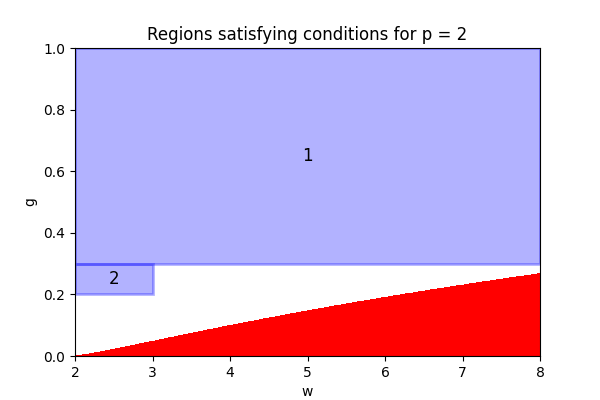
\includegraphics[width=\linewidth]{plotsexcom/plot_p_2.png}
        \caption{$p = 2$}
    \end{subfigure}
    \hfill
    \begin{subfigure}{0.32\textwidth}
        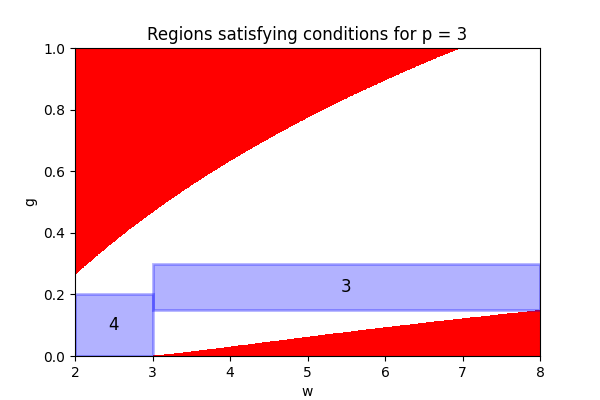
\includegraphics[width=\linewidth]{plotsexcom/plot_p_3.png}
        \caption{$p = 3$}
    \end{subfigure}
    \hfill
    \begin{subfigure}{0.32\textwidth}
        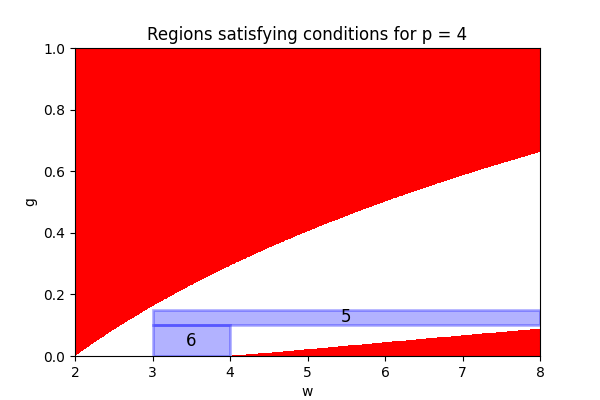
\includegraphics[width=\linewidth]{plotsexcom/plot_p_4.png}
        \caption{$p = 4$}
    \end{subfigure}
    \hfill
    \begin{subfigure}{0.32\textwidth}
       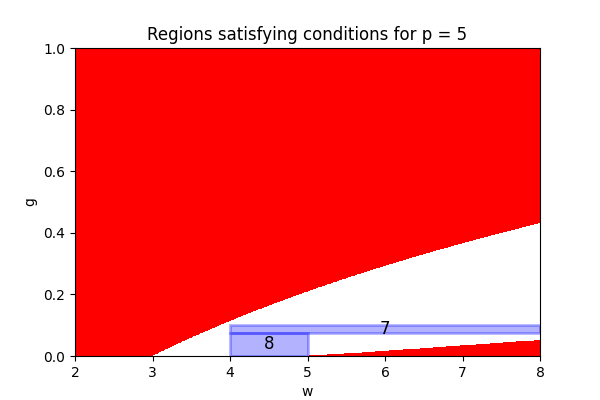
\includegraphics[width=\linewidth]{plotsexcom/plot_p_5.png}
        \caption{$p = 5$}
    \end{subfigure}
    \medskip
    \begin{subfigure}{0.32\textwidth}
        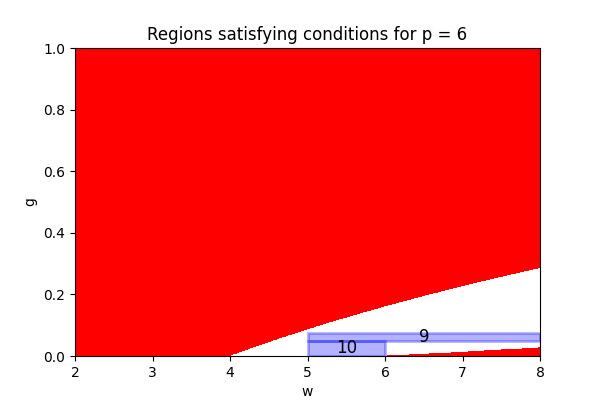
\includegraphics[width=\linewidth]{plotsexcom/plot_p_6.png}
        \caption{$p = 6$}
    \end{subfigure}
    \hfill
    \begin{subfigure}{0.32\textwidth}
        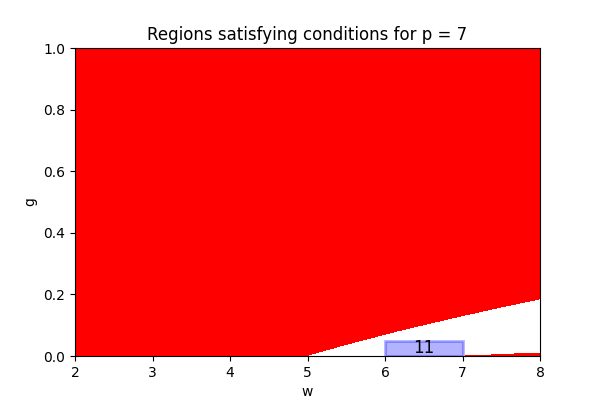
\includegraphics[width=\linewidth]{plotsexcom/plot_p_7.png}
        \caption{$p = 7$}
    \end{subfigure}
    \hfill
    \begin{subfigure}{0.32\textwidth}
        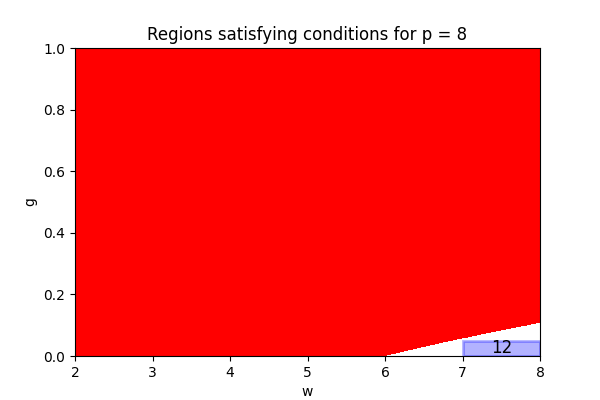
\includegraphics[width=\linewidth]{plotsexcom/plot_p_8.png}
        \caption{$p = 8$}
    \end{subfigure}
    \begin{subfigure}{0.32\textwidth}
        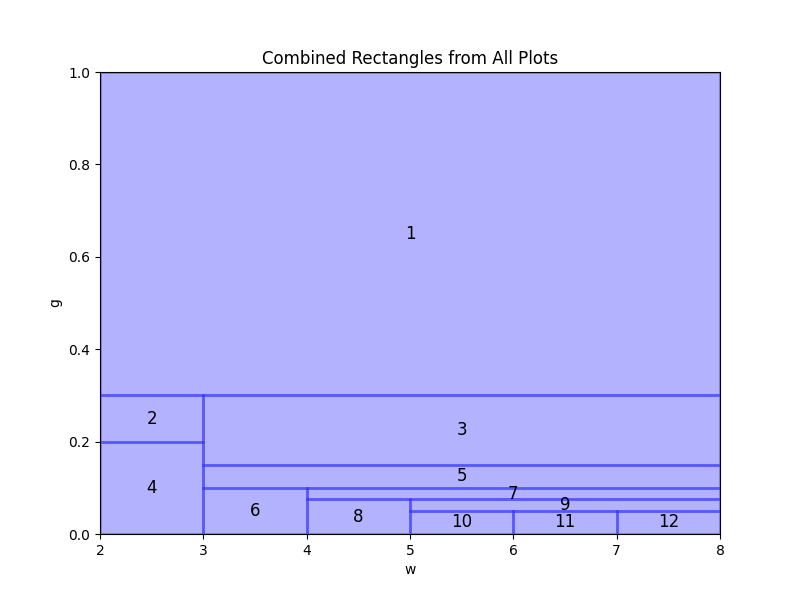
\includegraphics[width=\linewidth]{plotsexcom/rectanglesall.png}
        \caption{all rectangles}
    \end{subfigure}
    \caption{Comparative plots for different values of $p$.}
    \label{fig:all_plots}
\end{figure}

\begin{figure}
\center
\begin{tabular}{|c|c|c|c|c|c|c|}
\hline
Rectangle & $(w_1,\gamma_1)$ & $(w_2,\gamma_2)$ & $p$ & $p_{\max}(w_1,\gamma_1,p) $& $\alpha(w_1,\gamma_1,p)$ & $\beta(w_2,\gamma_2,p)$ \\
\hline
1 & $(2,1)$ & $(8,0.3)$ & 2 &1 & 2.00 & 1.89 \\
2 & $(2,0.3)$ & $(3,0.2)$ & 2 &4 & 1.49 & 1.41 \\
3 & $(3,0.3)$ & $(8,0.15)$ & 3 &6 & 1.79 & 1.99 \\
4 & $(2,0.2)$ & $(3,0)$ & 3 &7 & 1.91 & 2.00 \\
5 & $(3,0.15)$ & $(8,0.1)$ & 4 &14 & 1.98 & 1.92 \\
6 & $(3,0.1)$ & $(4,0)$ & 4 &22 & 1.90 & 2.00 \\
7 & $(4,0.1)$ & $(8,0.075)$ & 5 &29 & 1.97 & 1.83 \\
8 & $(4,0.075)$ & $(5,0)$ & 5 &40 & 1.93 & 2.00 \\
9 & $(5,0.075)$ & $(8,0.05)$ & 6 &50 & 1.98 & 1.82 \\
10 & $(5,0.05)$ & $(6,0)$ & 6 &80 & 1.93 & 2.00 \\
11 & $(6,0.05)$ & $(7,0)$ & 7 &96 & 1.96 & 2.00 \\
12 & $(7,0.05)$ & $(8,0)$ & 8 &111 & 1.98 & 2.00 \\
\hline
\end{tabular}
\label{fig.verif}
\caption{Verification of all extreme values in sub-areas}
\end{figure}



\textbf{Case 2}: $2 \leq w<8$. 
Let  $\alpha(w,\gamma,p)= \frac{a(w,\gamma,p)}{a_{min}(\gamma,p)}=\frac{w+p^{\gamma+1}}{w+1}$ and $\beta(w,\gamma,p)= \frac{\frac{w}{p}+p^\gamma}{\frac{w}{p^{\max}}+{p^{\max}}^\gamma}$. The objective is to show that for any couple $(w,\gamma)$, there exist a $p$ such that $\alpha(w,\gamma,p)\leq 2$ and $\beta(w,\gamma,p)\leq 2$.\\

We notice that $\alpha(w,\gamma,p)=1+\frac{p^{\gamma+1}-1}{w+1}$ increases with $\gamma$ and decreases with $w$. Similarly, if $p^{\max} \geq p$, $\beta(w,\gamma,p)$ increases with $w$ since a higher $w$ means a higher parallelism and therefore a higher ratio $\frac{t}{t_{min}}$, and decreases with $\gamma$ for the opposite reason. Finally, $p^{\max}$ increases with $w$ and decreases with $\gamma$. Therefore, if for a couple ($w,\gamma$), we are given $w_1 \leq w \leq w_2$, $\gamma_2 \leq \gamma \leq \gamma_1$ and $p$ such that $p^{\max}(w_1,\gamma_1) \geq p $, $\alpha(w_1,\gamma_1,p) \leq 2$ and $\beta(w_2,\gamma_2,p) \leq 2$, we will be assured $\alpha(w,\gamma,p) \leq 2$ and $\beta(w,\gamma,p) \leq 2$. We further illustrates this with Figure~\ref{fig:all_plots}: for each $p \in [2,8]$ we color in red the areas for which $\alpha(w,\gamma,p) > 2$ (top left area) and for which $\beta(w,\gamma,p) > 2$ (bottom right area). We will subdivise the zone $(w \in [2,8], \gamma \in [0,1])$ into $13$ subrectangles, each of them being assigned to one value of $p$. For instance, rectangle $3$ is assigned to $p=3$. To show that the rectangle doesn't cover any region that doesn't satisfy our conditions (in red), we simply need to verify the top left corner for $\alpha$, the bottom right corner for $\beta$, and $p \leq p^{\max}$ for the top left corner. All these verifications are summed up in the table in Figure~\ref{fig.verif} (note that the value are rounded but the $2.00$ are exactly $2$)\\



\textbf{Case 3}:  $w \geq 8$ and $\gamma \leq 0.1$
We use $p=\left\lceil w^{\frac{1}{\gamma+1}} \right\rceil$.
Then
\begin{align*}
\frac{t(p)}{t_{min}}&=\frac{\frac{w}{p}+p^\gamma}{t_{min}} \\
&\leq \frac{\frac{w}{ w^{\frac{1}{\gamma+1}}}+\left(  w^{\frac{1}{\gamma+1}} +1\right)^\gamma}{ \left( \gamma+1\right)\left( \frac{w}{\gamma} \right)^{\frac{\gamma}{\gamma+1}}} \\
&\leq \frac{w^{\frac{\gamma}{\gamma+1}}+w^{\frac{\gamma}{\gamma+1}}\left(1+\frac{1}{w^{\frac{1}{\gamma+1}}}\right)^\gamma}{ w^{\frac{\gamma}{\gamma+1}}\left( \frac{\gamma+1}{\gamma^{\frac{\gamma}{\gamma+1}}} \right)} \\
&\leq \frac{\gamma^{\frac{\gamma}{\gamma+1}}}{\gamma+1}\left(1+\left(1+\frac{1}{w^{\frac{1}{\gamma+1}}}\right)^\gamma\right) \\
&\leq \frac{1^{\frac{\gamma}{\gamma+1}}}{\gamma+1}\left(1+\left(1+\frac{1}{1^{\frac{1}{\gamma+1}}}\right)^\gamma\right)=\frac{2^\gamma+1}{\gamma+1} \\
\end{align*}
If we define $f(\gamma)=2^\gamma+1$ and $g(\gamma)=\gamma+1$, we have $f(0) \leq 2g(0)$ and $f(1) \leq g(1)$. $g$ is affine and $f$ is convexe thus $\forall \gamma, f(\gamma) \leq 2g(\gamma)$ and $\beta=\frac{t(p)}{t_{min}} \leq 2$.
\end{proof}

\begin{align*}
\frac{a(p)}{a_{min}} &= \frac{w+p^{\gamma+1}}{w+1} \\
&\leq \frac{w+\left(w^{\frac{1}{\gamma+1}}+1\right)^{\gamma+1}}{w+1}\\
&= \frac{w+w\left(1+w^{-\frac{1}{\gamma+1}}\right)^{\gamma+1}}{w+1}\\
&\leq \frac{w+w\left(1+w^{\frac{-1}{1.1}}\right)^{1.1}}{w+1}\\
\end{align*}
Because $(1+x)^a=\sum_{k=0}^\infty \frac{a(a-1)\cdots(a-k+1)}{k!}x^k$, with $1<a<2$ and $x<1$, we can upperbound the sum by the first three terms. Indeed the fourth term is negative and from there it's a sum that alternates positive and negative values of decreasing norm, hence $\sum_{k=3}^\infty \frac{a(a-1)\cdots(a-k+1)}{k!}x^k<0$, therefore $\left(1+w^{\frac{-1}{1.1}}\right)^{1.1} \leq 1+1.1w^{\frac{-1}{1.1}}+\frac{0.11}{2}w^{\frac{-2}{1.1}} \leq 1+1.1w^{\frac{-1}{1.1}}+0.1w^{-1}$. We conclude

\begin{align*}
\frac{a(p)}{a_{min}} &\leq \frac{w+w(1+1.1w^{\frac{-1}{1.1}}+0.1w^{-1})}{w+1} \\
&\leq \frac{2w+1.1w^{\frac{1}{11}}+0.1)}{w+1}\\
&= 2+\frac{1.1w^{\frac{1}{11}}-1.9}{w+1} \\
\end{align*}
If $w<\frac{1.9^{11}}{1.1}$, then $\frac{a(p)}{a_{min}} \leq 2$, otherwise $\frac{a(p)}{a_{min}} \leq 2+1.1w^{-10/11} \leq 2+1.9^{-10} < 2.002$. In both case $\alpha<2.002$.

\textbf{Case 4}:  $w \geq 8$ and $\gamma > 0.1$.
We use $p=\left\lfloor w^{\frac{1}{\gamma+1}} \right\rfloor$.

\begin{align*}
\frac{t(p)}{t_{min}}&=\frac{\frac{w}{p}+p^\gamma}{t_{min}} \\
&\leq \frac{\frac{w}{ w^{\frac{1}{\gamma+1}}-1}+\left( w^{\frac{1}{\gamma+1}}\right)^\gamma}{ \left( \gamma+1\right)\frac{w}{\gamma} ^{\frac{\gamma}{\gamma+1}}} \\
&= \frac{\gamma^{\frac{\gamma}{\gamma+1}}}{\gamma+1} \frac{\frac{w^{\frac{\gamma}{\gamma+1}}}{1-w^\frac{-1}{\gamma+1}}+w^{\frac{\gamma}{\gamma+1}}}{ w^{\frac{\gamma}{\gamma+1}}} \\
&\leq \frac{1}{\gamma+1}\left( \frac{1}{1-w^\frac{-1}{\gamma+1}}+1\right) \\
\end{align*}
Since the function decreases with $\gamma$ and $w$, we can replace $w$ by $8$ and $\gamma$ by $0.1$ which gives $\beta<1.98$.

Finally, 

\begin{align*}
\frac{a(p)}{a_{min}} &= \frac{w+p^{\gamma+1}}{w+1} \\
&\leq \frac{w+\left(w^{\frac{1}{\gamma+1}}\right)^{\gamma+1}}{w+1}\leq \frac{2w}{w+1}<2\\
\end{align*}

\FloatBarrier 
\newpage

\section{Appendix : Proof of General ratio}


\begin{lemma}\label{lem.general}
For any task that follows the general model, there exists a processor allocation that achieves $\alpha^{\GEN}=2.018
$ and $\beta^{\GEN}=2.018$.
\end{lemma}

\begin{proof}
If we allow the processor allocation to take non-integer values and assuming unbounded $\bar{p}$, the execution time function $t(p)$ would be minimized at $p^*=\sqrt{w'}$. Thus, the minimum execution time should satisfy $t^{\min}\ge c(2\sqrt{w'}+d'-1)$. Note that this bound will hold true regardless of the value of $\bar{p}$: it is obviously true if $\bar{p} \ge p^*$, otherwise $t^{\min}$ is achieved at $\bar{p}$, with a value also higher than $c(2\sqrt{w'}+d'-1)$.
Furthermore, the minimum area is obtained with one processor, i.e., $a^{\min} = a(1) = c(w'+d')$.

Recall that $p^{\max}$ denotes the number of processors that minimizes the execution time, i.e., $t(p^{\max}) = t^{\min}$. Clearly, we have either $p^{\max}=\bar{p}$ or $\lfloor \sqrt{w'} \rfloor \leq p^{\max} \leq \lceil \sqrt{w'} \rceil$.

We consider three cases.

\textbf{Case 1}: $w'\leq 4$ or $\bar{p}=1$. In this case, it must be that $p^{\max}\leq 2$. We can then set $p = 1$, and get $\frac{a(p)}{a^{\min}}=1$ and $\frac{t(p)}{t^{\min}} \leq 2$.

\textbf{Case 2}: $4<w'\leq 800$ and $d>800$.In this case, we chose $p=1$ since $t_{min}>d>w'$ and $t(1)=w+d<2t_{min}$.



\begin{figure}[ht]
    \centering
    \begin{subfigure}{0.32\textwidth}
        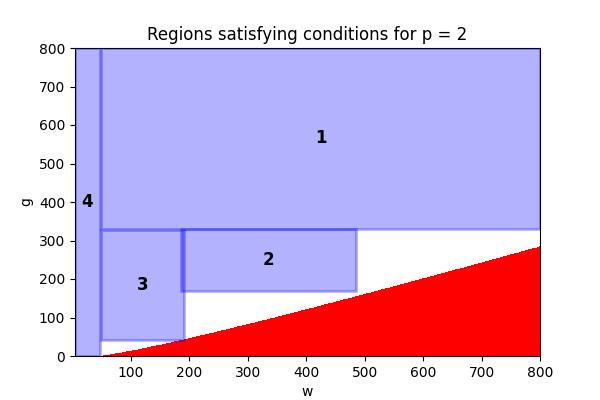
\includegraphics[width=\linewidth]{plotsgen/plot_p_2.png}
        \caption{$p = 2$}
    \end{subfigure}
    \hfill
    \begin{subfigure}{0.32\textwidth}
        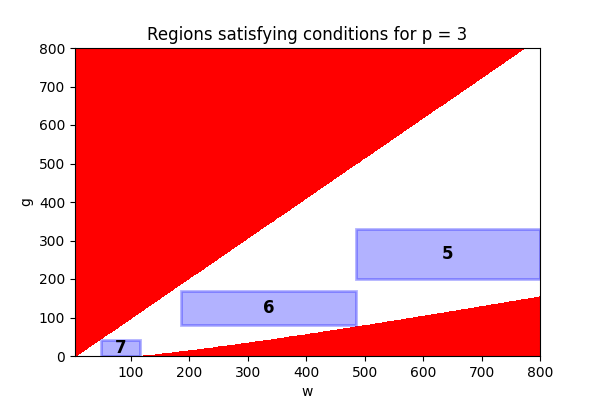
\includegraphics[width=\linewidth]{plotsgen/plot_p_3.png}
        \caption{$p = 3$}
    \end{subfigure}
    \hfill
    \begin{subfigure}{0.32\textwidth}
        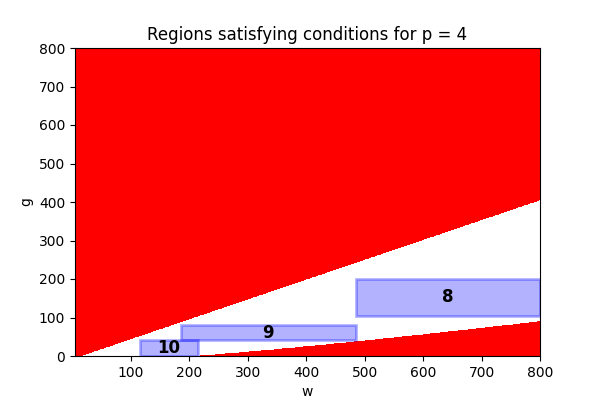
\includegraphics[width=\linewidth]{plotsgen/plot_p_4.png}
        \caption{$p = 4$}
    \end{subfigure}
    \hfill
    \begin{subfigure}{0.32\textwidth}
        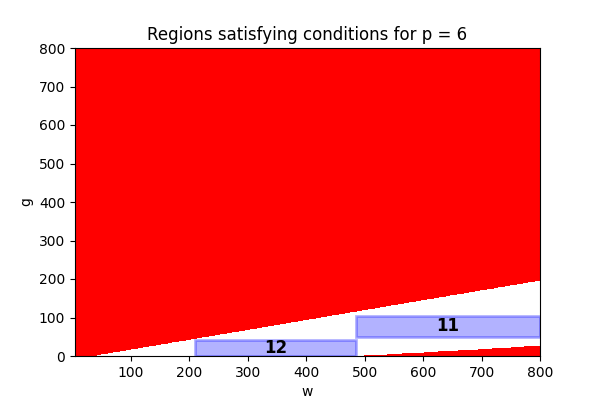
\includegraphics[width=\linewidth]{plotsgen/plot_p_6.png}
        \caption{$p = 6$}
    \end{subfigure}
    \hfill
    \begin{subfigure}{0.32\textwidth}
        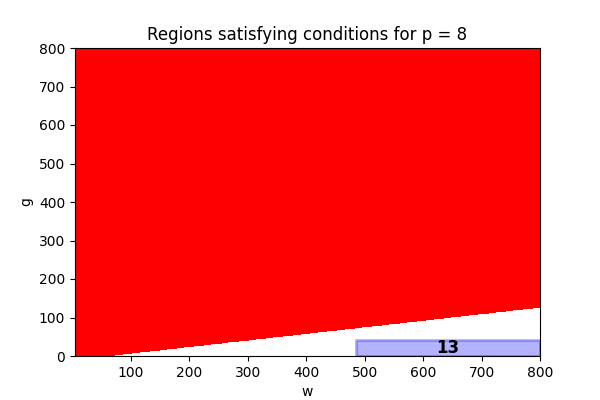
\includegraphics[width=\linewidth]{plotsgen/plot_p_8.png}
        \caption{$p = 8$}
    \end{subfigure}
    \begin{subfigure}{0.32\textwidth}
        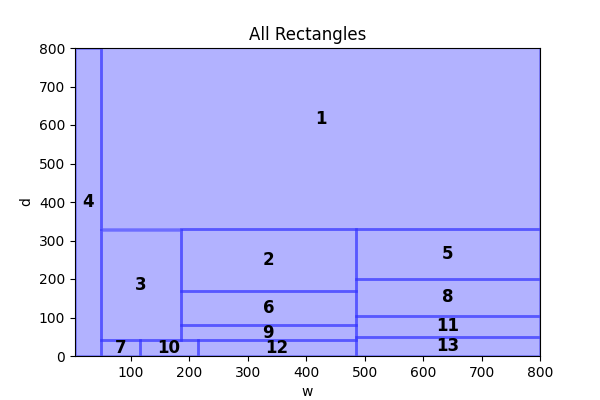
\includegraphics[width=\linewidth]{plotsgen/rectanglesall.png}
        \caption{all rectangles}
    \end{subfigure}
    \caption{Comparative plots for different values of $p$.}
    \label{fig:all_plotsgen}
\end{figure}

\begin{figure}
\center
\begin{tabular}{|c|c|c|c|c|c|c|}
\hline
Rectangle & $(w_1,\gamma_1)$ & $(w_2,\gamma_2)$ & $p$ & $p_{min}(w_1,\gamma_1,p) $& $f(w_1,\gamma_1,p)$ & $g(w_2,\gamma_2,p)$ \\
\hline
1 & $(49,800)$ & $(800,330)$ & 2 &7 & 1.945 & 1.896 \\
2 & $(185,330)$ & $(485,170)$ & 2 &14 & 1.645 & 1.941 \\
3 & $(49,330)$ & $(185,42)$ & 2 &7 & 1.876 & 1.986 \\
4 & $(4,800)$ & $(49,0)$ & 2 &2 & 1.998 & 1.962 \\
5 & $(485,330)$ & $(800,200)$ & 3 &22 & 1.817 & 1.834 \\
6 & $(185,170)$ & $(485,80)$ & 3 &14 & 1.975 & 1.980 \\
7 & $(49,42)$ & $(115,0)$ & 3 &7 & 1.989 & 1.972 \\
8 & $(485,200)$ & $(800,105)$ & 4 &22 & 1.893 & 1.918 \\
9 & $(185,80)$ & $(485,42)$ & 4 &14 & 1.951 & 1.955 \\
10 & $(115,42)$ & $(215,0)$ & 4 &11 & 1.879 & 2.003 \\
11 & $(485,105)$ & $(800,50)$ & 6 &22 & 1.941 & 1.784 \\
12 & $(215,42)$ & $(485,0)$ & 6 &15 & 1.934 & 1.994 \\
13 & $(485,50)$ & $(800,0)$ & 8 &22 & 1.759 & 1.925 \\
\hline
\end{tabular}
\caption{Verification of all extreme values in sub-areas}
\label{fig.verif2}
\end{figure}
\textbf{Case 3}: Here we will first assume $\bar{p}$ is unbounded. Similarly to previous appendix, we notice that $\alpha(w,d,p)=1+\frac{(p-1)(d+p)}{w+d}$ decreases with $w$. When derivating subject to $d$, we get $\frac{\partial\alpha(w,d,p)}{\partial d}=\frac{(w-p)(p-1)}{(w+d)^2}>0$ if $w>p$. Similarly, if $p^{\max} \geq p$, $\beta(w,d,p)$ increases with $w$ since a higher $w$ means a higher parallelism and therefore a higher ratio $\frac{t}{t_{min}}$, and decreases with $d$ for the opposite reason. Finally, $p^{\max}$ increases with $w$ and decreases with $d$. 

Therefore, if for a couple ($w,d$), we are given $w_1 \leq w \leq w_2$, $d_2 \leq d \leq d_1$ and $p$ such that $p^{\max}(w_1,d_1) \geq p $, $w_1 \geq p$, $\alpha(w_1,d_1,p) \leq 2$ and $\beta(w_2,d_2,p) \leq 2$, we will be assured $\alpha(w,d,p) \leq 2$ and $\beta(w,d,p) \leq 2$. We further illustrates this with Figure~\ref{fig:all_plots}: for each $p \in [2,8]$ we color in red the areas for which $\alpha(w,d,p) > 2$ (top left area) and for which $\beta(w,d,p) > 2$ (bottom right area). Again, we will subdivise the zone $(w \in [4,800], d \in [0,800])$ into $12$ subrectangles, each of them being assigned to one value of $p$. For instance, rectangle $5$ is assigned to $p=3$. To show that the rectangle doesn't cover any region that doesn't satisfy our conditions (in red), we simply need to verify the top left corner for $\alpha$, the bottom right corner for $\beta$, and $p \leq p^{\max}$ for the top left corner. All these verifications are summed up in the table in Figure~\ref{fig.verif2}.\\

We have shown that if $\bar{p}$ is unbounded, there exists $p'$ such that $\frac{t(p')}{t_{min}} \leq 2.018$ and $\frac{a(p')}{a_{min}}\leq 2.018$. If $\bar{p}>p'$, then we just fix $p=\bar{p}=p^{\max}$, the area will decrease and we get $t(p)=t_{min}$

\textbf{Case 4}: $w'>800$ and $\bar{p}\geq 2$. \LP{This derivation is from ICPP24 paper, except we use $800$ instead of $49$ for better bounds}In this case, we will set $p=\min\left(\left\lfloor \frac{w'+d'}{\sqrt{w'}+d'} +\frac{1}{2}\right\rfloor,\bar{p}\right)$ and get:
\begin{align*}
\frac{a(p)}{a^{\min}} &= \frac{w'+p(d'+p-1)}{w'+d'} \\
&\leq \frac{w'+\left(\frac{w'+d'}{\sqrt{w'}+d'}+\frac{1}{2}\right)\left(d'+\frac{w'+d'}{\sqrt{w'}+d'}-\frac{1}{2}\right)}{w'+d'} \\
&= \frac{w'+\frac{d'}{2}-\frac{1}{4}+\frac{w'+d'}{\sqrt{w'}+d'}\left(d'+\frac{w'+d'}{\sqrt{w'}+d'} \right)}{w'+d'} \\
&\le \frac{w'+d'+\frac{w'+d'}{\sqrt{w'}+d'}\left(d'+\frac{w'+d'}{\sqrt{w'}+d'} \right)}{w'+d'} \\
&= 1+\frac{d'(\sqrt{w'}+d')+w'+d'}{(\sqrt{w'}+d')^2} \\
&=1+\frac{d'^2+d'\sqrt{w'}+d'+w'}{d'^2+2d'\sqrt{w'}+w'} \\
&\leq 2 \ .
\end{align*}
The last inequality above comes from $w'>1$ and $d'\geq 0$.

Since $w'>1$, we get $t^{\min}\ge c(2\sqrt{w'}+d'-1)>c(\sqrt{w'}+d')$. To derive the execution time ratio, we further consider two subcases.
\begin{itemize}
\item If $p=\left\lfloor \frac{w'+d'}{\sqrt{w'}+d'} +\frac{1}{2}\right\rfloor$, then $p\geq \frac{w'+d'}{\sqrt{w'}+d'} - \frac{1}{2} \geq \frac{w'-\frac{1}{2}\sqrt{w'}}{\sqrt{w'}+d'}$. We can then get:
\begin{align*}
\frac{t(p)}{t^{\min}} &\leq \frac{\frac{w'}{p}+d'+p-1}{\sqrt{w'}+d'} \\
&\leq \frac{\frac{w'(\sqrt{w'}+d')}{w'-\frac{1}{2}\sqrt{w'}}}{\sqrt{w'}+d'}+\frac{d'+\frac{w'+d'}{\sqrt{w'}+d'}}{\sqrt{w'}+d'} \\
&\leq \frac{1}{1-\frac{1}{2\sqrt{w'}}}+\frac{d'(\sqrt{w'}+d')+w'+d'}{(\sqrt{w'}+d')^2}\\
&\leq \frac{1}{1-\frac{1}{2\sqrt{w'}}}+1
\end{align*}
For the last inequality, we recognize the same term we had when bounding the area ratio, which is at most $1$. Finally, the last expression above decreases with $w'$, so using $w'>800$, we get $\frac{t(p)}{t^{\min}} \le \frac{1}{1-\frac{1}{\sqrt{800}}}+1<2.018$.
\item If $p = \bar{p} < \left\lfloor \frac{w'+d'}{\sqrt{w'}+d'} +\frac{1}{2}\right\rfloor$, and since $\bar{p}$ is an integer, then it is necessarily the case that $\bar{p} \le \left\lfloor \frac{w'+d'}{\sqrt{w'}+d'} +\frac{1}{2}\right\rfloor - 1 \le \frac{w'+d'}{\sqrt{w'}+d'} \leq \sqrt{w'}$ (because $w'>1$). Therefore, we should also have $p^{\max} = \bar{p} = p$, and thus $\frac{t(p)}{t^{\min}}=1$. \qedhere
\end{itemize}
\end{proof}

\FloatBarrier 
\newpage
\section{Appendix : Full Experimental Results}

\subsection{Lines Figures}
\begin{figure}[htbp]
\centering
\begin{subfigure}[b]{0.32\textwidth}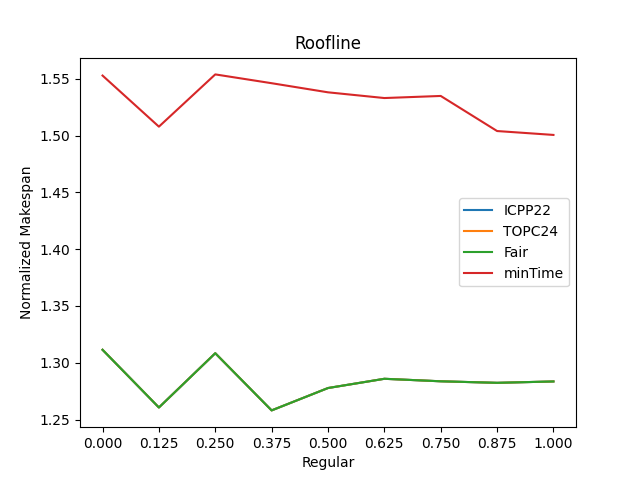
\includegraphics[width=\textwidth]{Results/Regular/Regular_Roofline}\caption{Roofline}\label{fig:lines_figures_Regular_Roofline}\end{subfigure}
\hfill
\begin{subfigure}[b]{0.32\textwidth}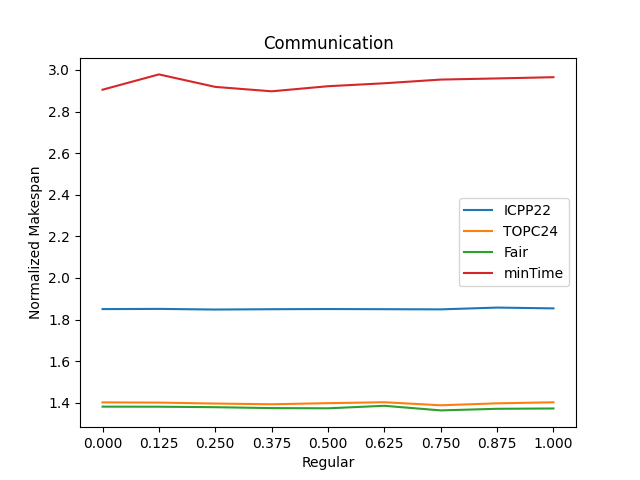
\includegraphics[width=\textwidth]{Results/Regular/Regular_Communication}\caption{Communication}\label{fig:lines_figures_Regular_Communication}\end{subfigure}
\hfill
\begin{subfigure}[b]{0.32\textwidth}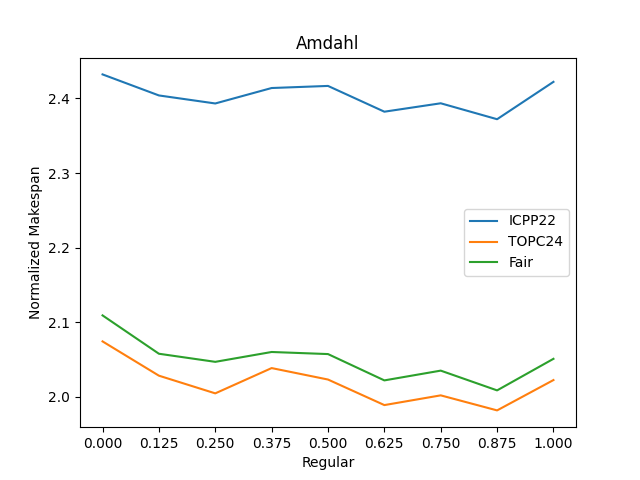
\includegraphics[width=\textwidth]{Results/Regular/Regular_Amdahl}\caption{Amdahl}\label{fig:lines_figures_Regular_Amdahl}\end{subfigure}
\\[2ex]
\begin{subfigure}[b]{0.32\textwidth}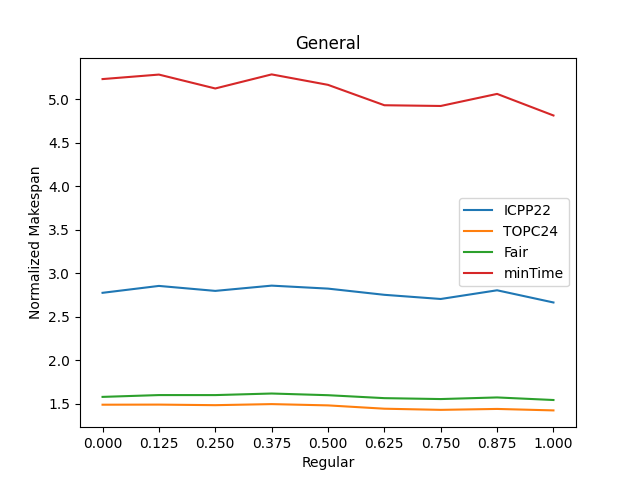
\includegraphics[width=\textwidth]{Results/Regular/Regular_General}\caption{General}\label{fig:lines_figures_Regular_General}\end{subfigure}
\hfill
\begin{subfigure}[b]{0.32\textwidth}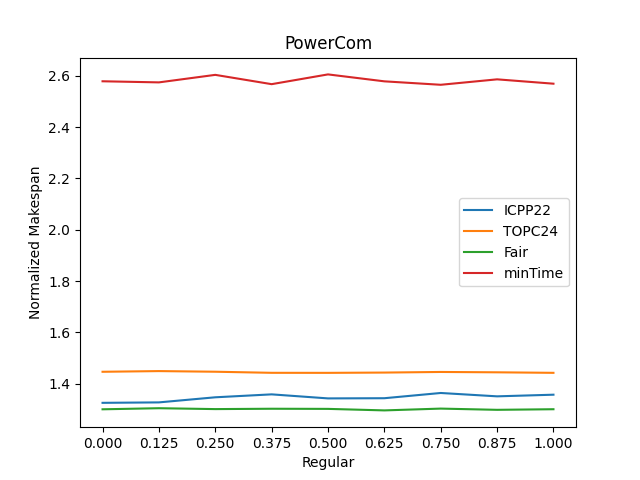
\includegraphics[width=\textwidth]{Results/Regular/Regular_PowerCom}\caption{PowerCom}\label{fig:lines_figures_Regular_PowerCom}\end{subfigure}
\hfill
\caption{Lines Figure for Regular}
\label{fig:lines_figures_Regular}
\end{figure}
\begin{figure}[htbp]
\centering
\begin{subfigure}[b]{0.32\textwidth}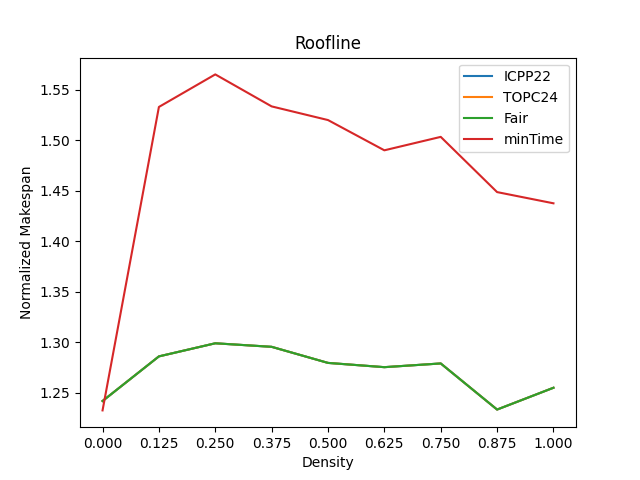
\includegraphics[width=\textwidth]{Results/Density/Density_Roofline}\caption{Roofline}\label{fig:lines_figures_Density_Roofline}\end{subfigure}
\hfill
\begin{subfigure}[b]{0.32\textwidth}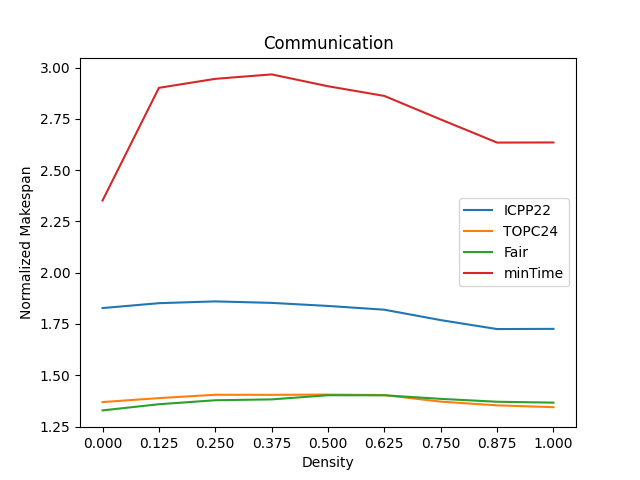
\includegraphics[width=\textwidth]{Results/Density/Density_Communication}\caption{Communication}\label{fig:lines_figures_Density_Communication}\end{subfigure}
\hfill
\begin{subfigure}[b]{0.32\textwidth}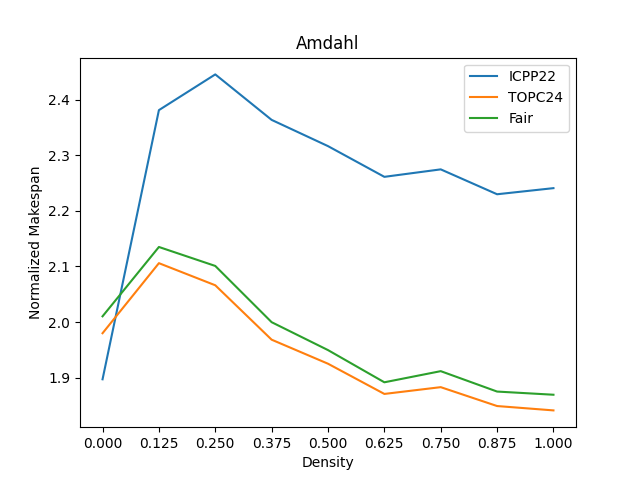
\includegraphics[width=\textwidth]{Results/Density/Density_Amdahl}\caption{Amdahl}\label{fig:lines_figures_Density_Amdahl}\end{subfigure}
\\[2ex]
\begin{subfigure}[b]{0.32\textwidth}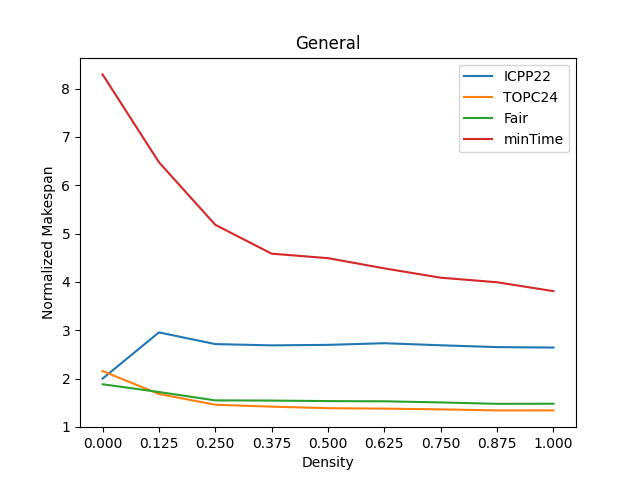
\includegraphics[width=\textwidth]{Results/Density/Density_General}\caption{General}\label{fig:lines_figures_Density_General}\end{subfigure}
\hfill
\begin{subfigure}[b]{0.32\textwidth}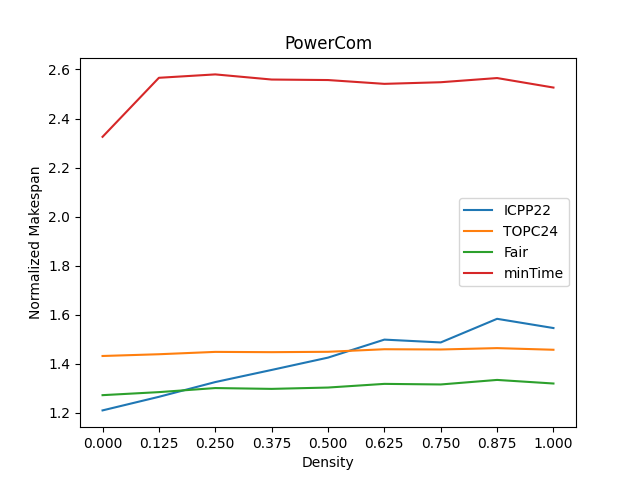
\includegraphics[width=\textwidth]{Results/Density/Density_PowerCom}\caption{PowerCom}\label{fig:lines_figures_Density_PowerCom}\end{subfigure}
\hfill
\caption{Lines Figure for Density}
\label{fig:lines_figures_Density}
\end{figure}
\begin{figure}[htbp]
\centering
\begin{subfigure}[b]{0.32\textwidth}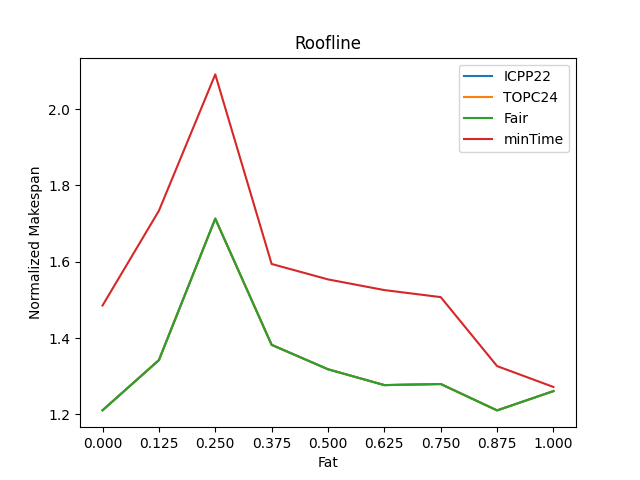
\includegraphics[width=\textwidth]{Results/Fat/Fat_Roofline}\caption{Roofline}\label{fig:lines_figures_Fat_Roofline}\end{subfigure}
\hfill
\begin{subfigure}[b]{0.32\textwidth}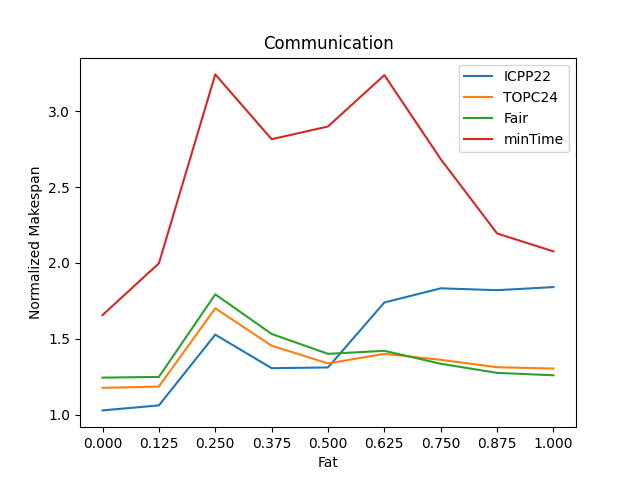
\includegraphics[width=\textwidth]{Results/Fat/Fat_Communication}\caption{Communication}\label{fig:lines_figures_Fat_Communication}\end{subfigure}
\hfill
\begin{subfigure}[b]{0.32\textwidth}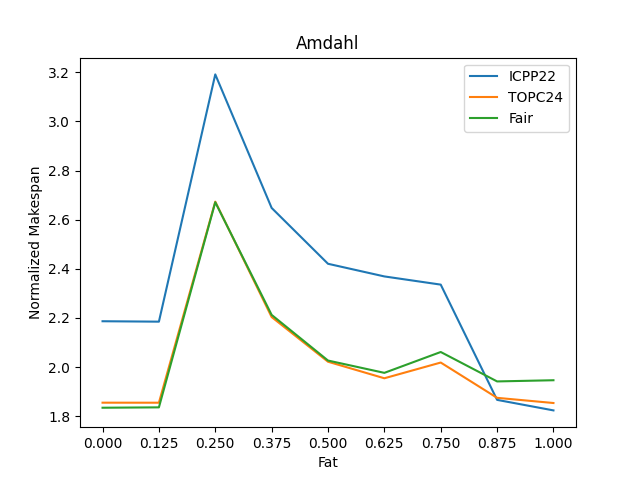
\includegraphics[width=\textwidth]{Results/Fat/Fat_Amdahl}\caption{Amdahl}\label{fig:lines_figures_Fat_Amdahl}\end{subfigure}
\\[2ex]
\begin{subfigure}[b]{0.32\textwidth}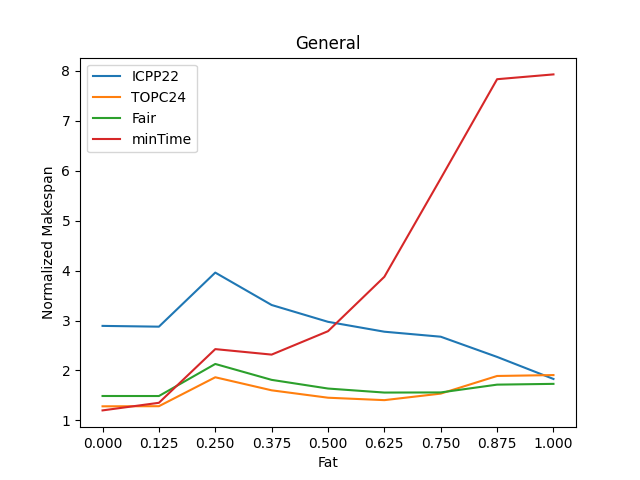
\includegraphics[width=\textwidth]{Results/Fat/Fat_General}\caption{General}\label{fig:lines_figures_Fat_General}\end{subfigure}
\hfill
\begin{subfigure}[b]{0.32\textwidth}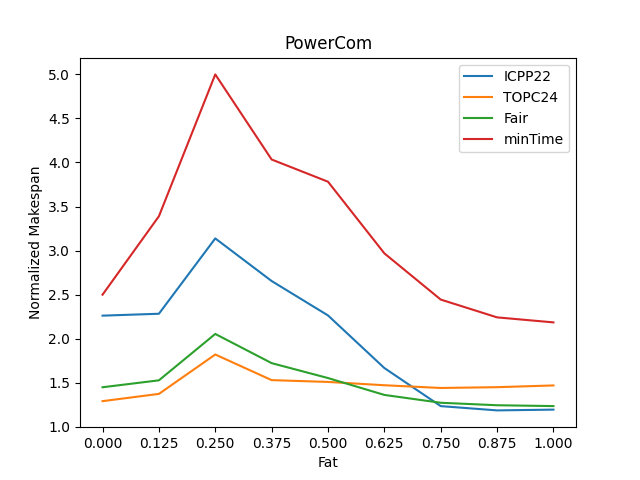
\includegraphics[width=\textwidth]{Results/Fat/Fat_PowerCom}\caption{PowerCom}\label{fig:lines_figures_Fat_PowerCom}\end{subfigure}
\hfill
\caption{Lines Figure for Fat}
\label{fig:lines_figures_Fat}
\end{figure}
\begin{figure}[htbp]
\centering
\begin{subfigure}[b]{0.32\textwidth}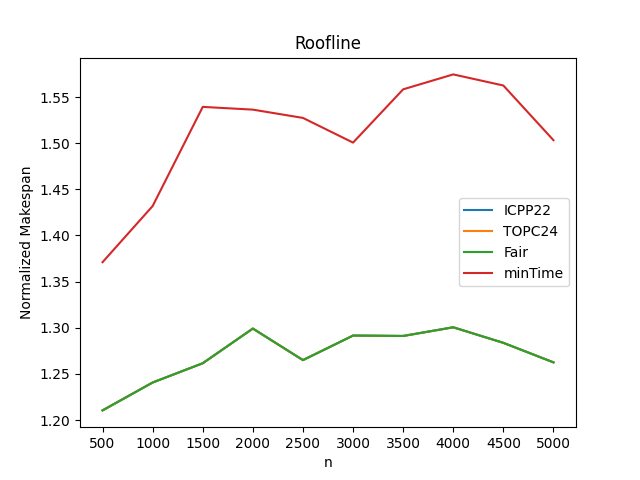
\includegraphics[width=\textwidth]{Results/n/n_Roofline}\caption{Roofline}\label{fig:lines_figures_n_Roofline}\end{subfigure}
\hfill
\begin{subfigure}[b]{0.32\textwidth}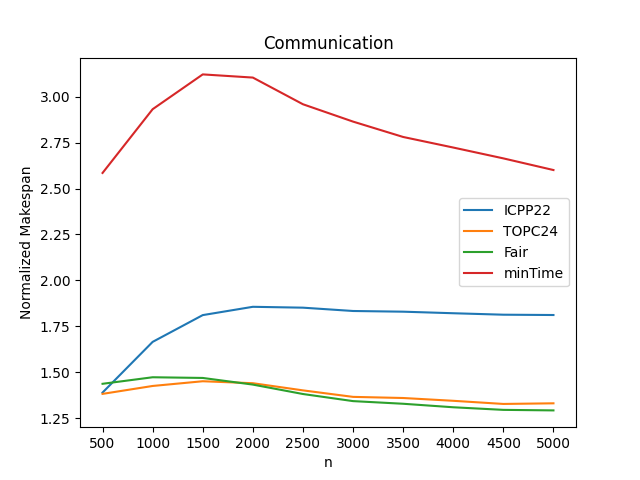
\includegraphics[width=\textwidth]{Results/n/n_Communication}\caption{Communication}\label{fig:lines_figures_n_Communication}\end{subfigure}
\hfill
\begin{subfigure}[b]{0.32\textwidth}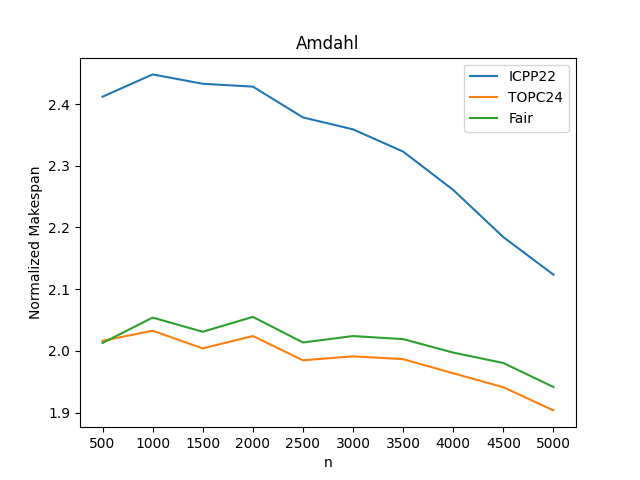
\includegraphics[width=\textwidth]{Results/n/n_Amdahl}\caption{Amdahl}\label{fig:lines_figures_n_Amdahl}\end{subfigure}
\\[2ex]
\begin{subfigure}[b]{0.32\textwidth}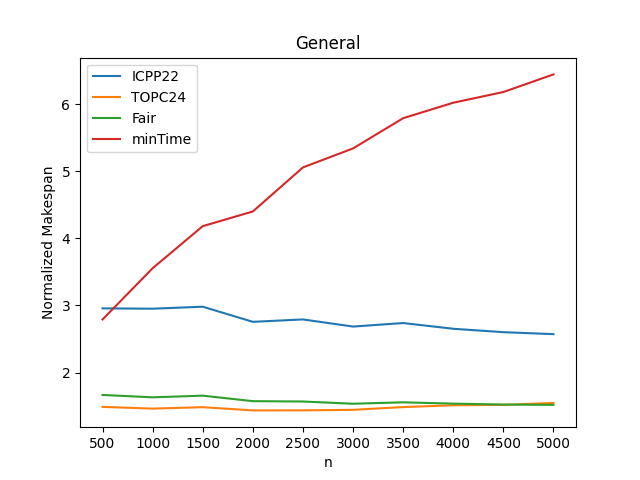
\includegraphics[width=\textwidth]{Results/n/n_General}\caption{General}\label{fig:lines_figures_n_General}\end{subfigure}
\hfill
\begin{subfigure}[b]{0.32\textwidth}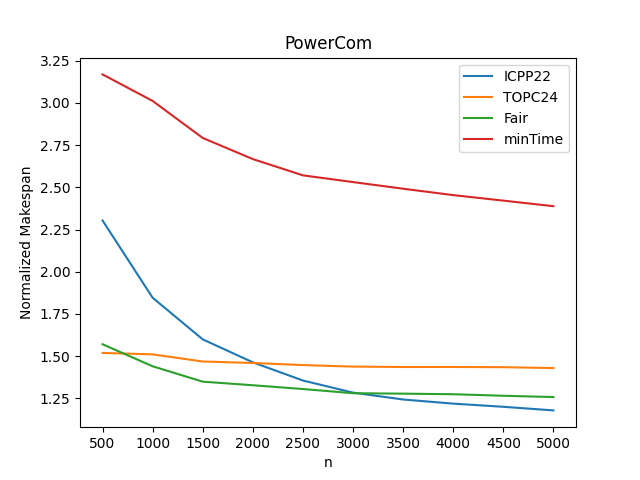
\includegraphics[width=\textwidth]{Results/n/n_PowerCom}\caption{PowerCom}\label{fig:lines_figures_n_PowerCom}\end{subfigure}
\hfill
\caption{Lines Figure for n}
\label{fig:lines_figures_n}
\end{figure}
\begin{figure}[htbp]
\centering
\begin{subfigure}[b]{0.32\textwidth}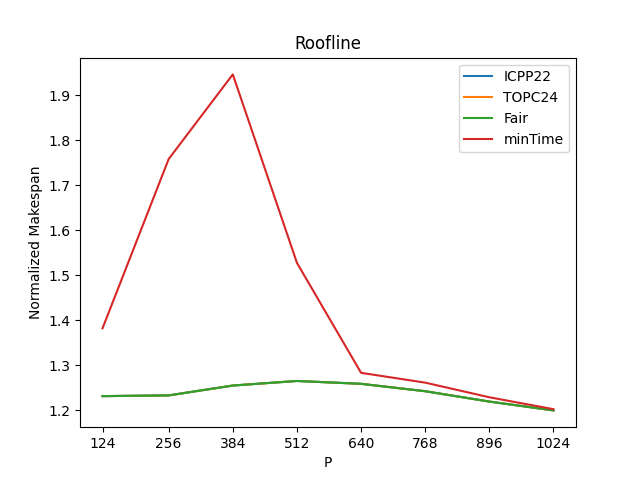
\includegraphics[width=\textwidth]{Results/P/P_Roofline}\caption{Roofline}\label{fig:lines_figures_P_Roofline}\end{subfigure}
\hfill
\begin{subfigure}[b]{0.32\textwidth}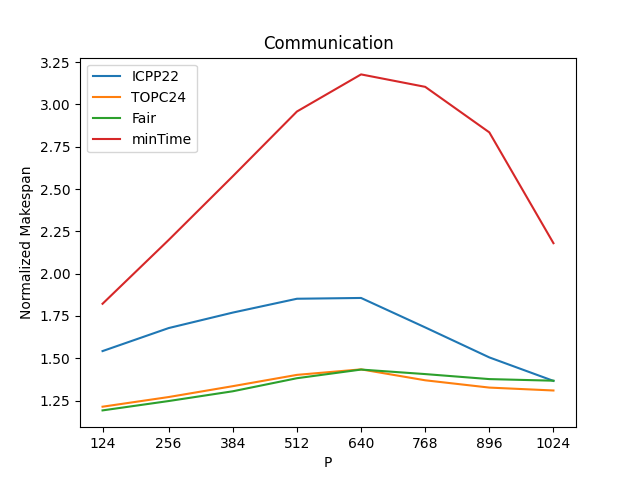
\includegraphics[width=\textwidth]{Results/P/P_Communication}\caption{Communication}\label{fig:lines_figures_P_Communication}\end{subfigure}
\hfill
\begin{subfigure}[b]{0.32\textwidth}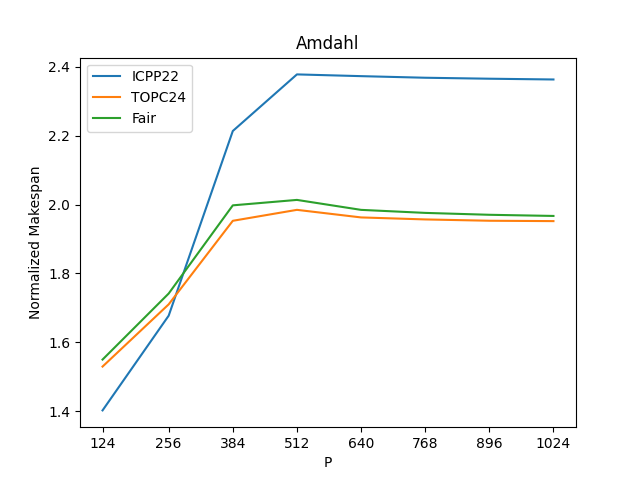
\includegraphics[width=\textwidth]{Results/P/P_Amdahl}\caption{Amdahl}\label{fig:lines_figures_P_Amdahl}\end{subfigure}
\\[2ex]
\begin{subfigure}[b]{0.32\textwidth}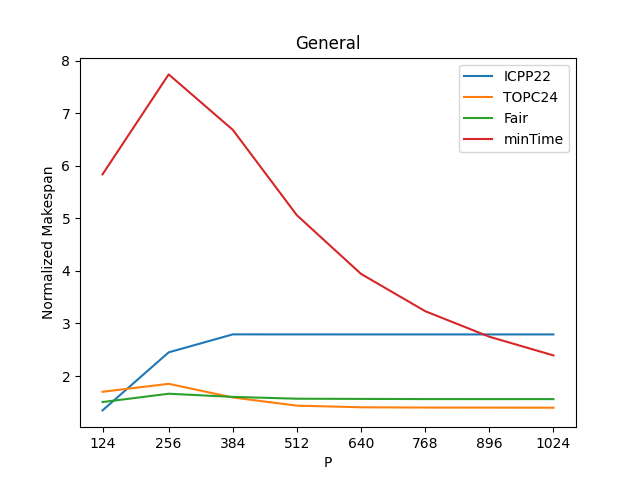
\includegraphics[width=\textwidth]{Results/P/P_General}\caption{General}\label{fig:lines_figures_P_General}\end{subfigure}
\hfill
\begin{subfigure}[b]{0.32\textwidth}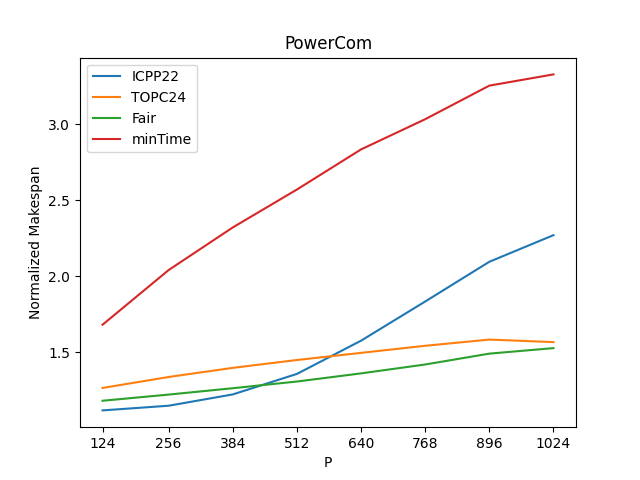
\includegraphics[width=\textwidth]{Results/P/P_PowerCom}\caption{PowerCom}\label{fig:lines_figures_P_PowerCom}\end{subfigure}
\hfill
\caption{Lines Figure for P}
\label{fig:lines_figures_P}
\end{figure}
\begin{figure}[htbp]
\centering
\begin{subfigure}[b]{0.32\textwidth}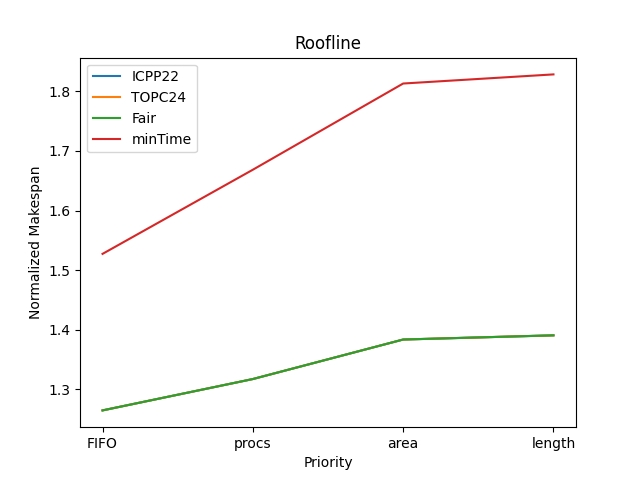
\includegraphics[width=\textwidth]{Results/Priority/Priority_Roofline}\caption{Roofline}\label{fig:lines_figures_Priority_Roofline}\end{subfigure}
\hfill
\begin{subfigure}[b]{0.32\textwidth}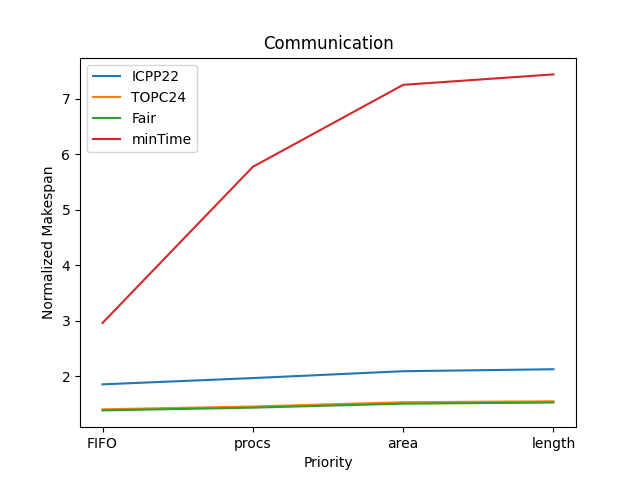
\includegraphics[width=\textwidth]{Results/Priority/Priority_Communication}\caption{Communication}\label{fig:lines_figures_Priority_Communication}\end{subfigure}
\hfill
\begin{subfigure}[b]{0.32\textwidth}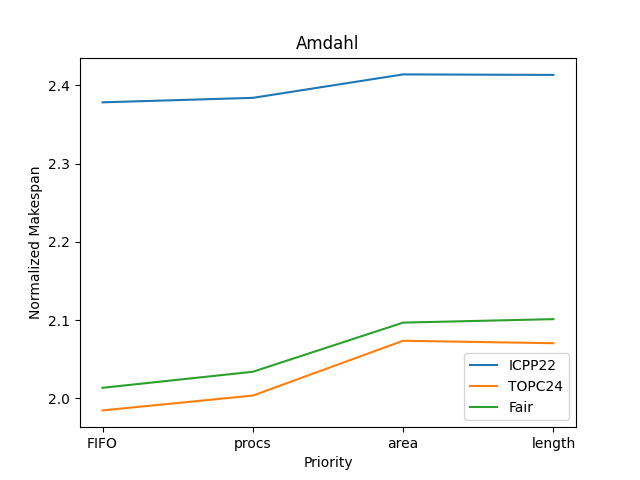
\includegraphics[width=\textwidth]{Results/Priority/Priority_Amdahl}\caption{Amdahl}\label{fig:lines_figures_Priority_Amdahl}\end{subfigure}
\\[2ex]
\begin{subfigure}[b]{0.32\textwidth}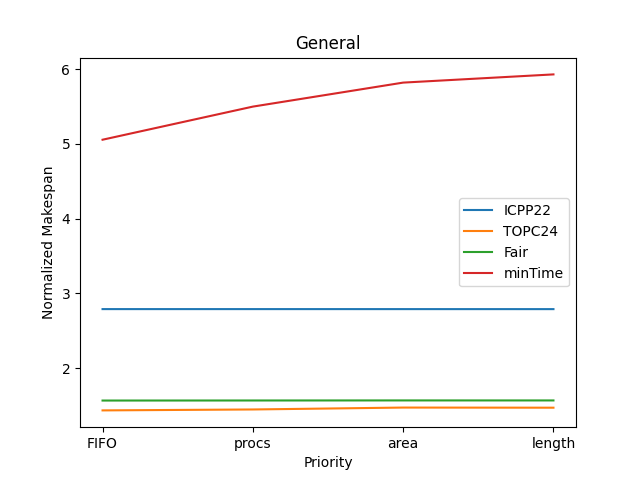
\includegraphics[width=\textwidth]{Results/Priority/Priority_General}\caption{General}\label{fig:lines_figures_Priority_General}\end{subfigure}
\hfill
\begin{subfigure}[b]{0.32\textwidth}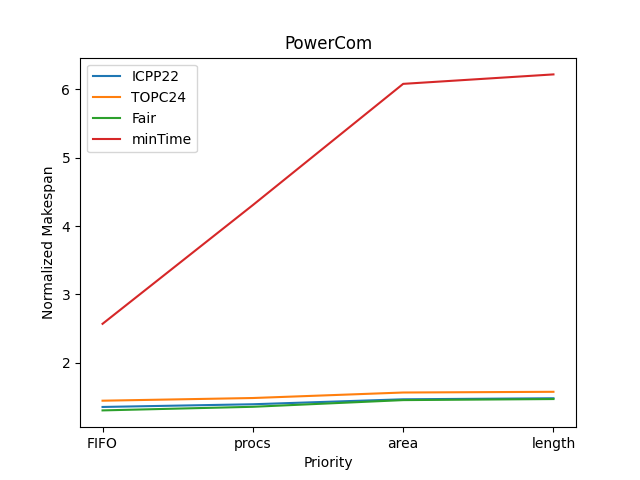
\includegraphics[width=\textwidth]{Results/Priority/Priority_PowerCom}\caption{PowerCom}\label{fig:lines_figures_Priority_PowerCom}\end{subfigure}
\hfill
\caption{Lines Figure for Priority}
\label{fig:lines_figures_Priority}
\end{figure}
\begin{figure}[htbp]
\centering
\begin{subfigure}[b]{0.32\textwidth}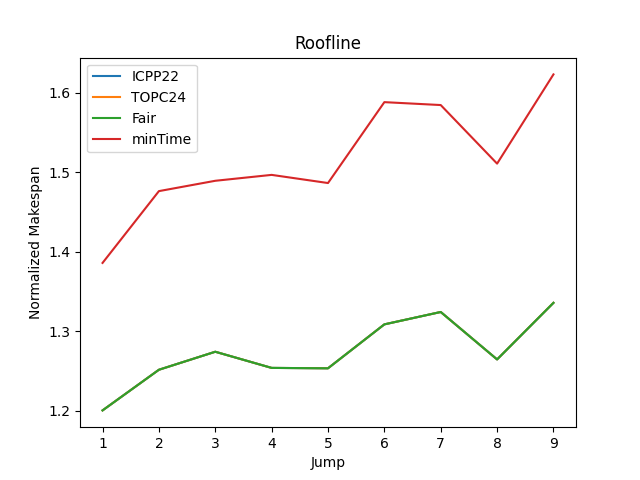
\includegraphics[width=\textwidth]{Results/Jump/Jump_Roofline}\caption{Roofline}\label{fig:lines_figures_Jump_Roofline}\end{subfigure}
\hfill
\begin{subfigure}[b]{0.32\textwidth}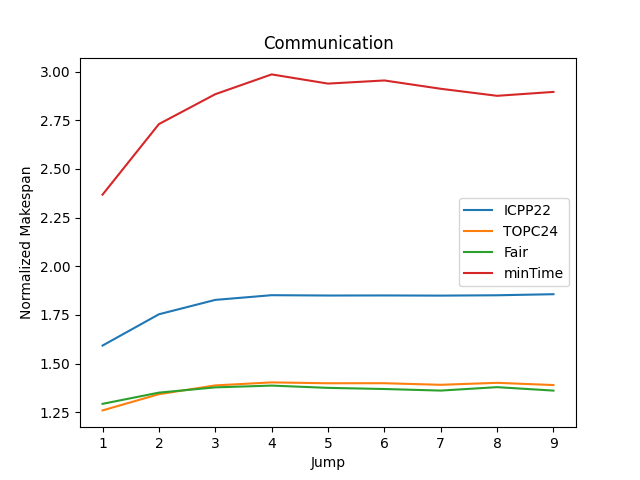
\includegraphics[width=\textwidth]{Results/Jump/Jump_Communication}\caption{Communication}\label{fig:lines_figures_Jump_Communication}\end{subfigure}
\hfill
\begin{subfigure}[b]{0.32\textwidth}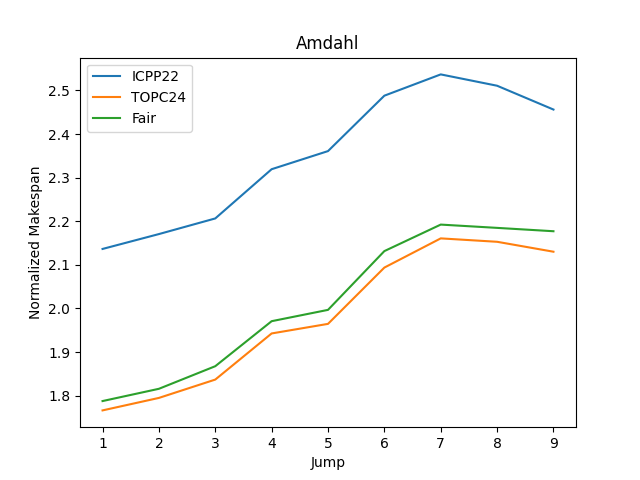
\includegraphics[width=\textwidth]{Results/Jump/Jump_Amdahl}\caption{Amdahl}\label{fig:lines_figures_Jump_Amdahl}\end{subfigure}
\\[2ex]
\begin{subfigure}[b]{0.32\textwidth}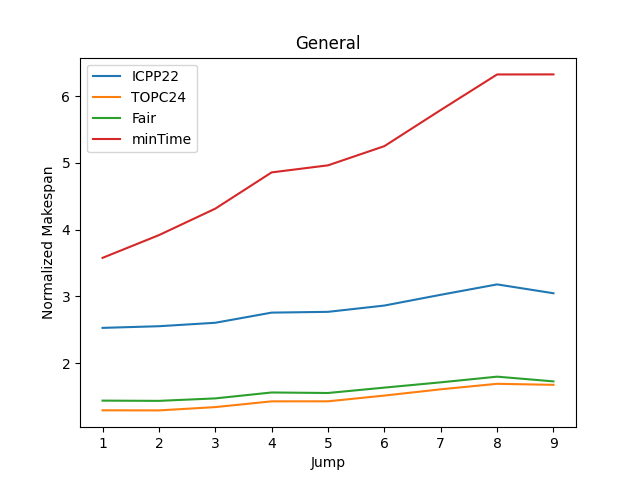
\includegraphics[width=\textwidth]{Results/Jump/Jump_General}\caption{General}\label{fig:lines_figures_Jump_General}\end{subfigure}
\hfill
\begin{subfigure}[b]{0.32\textwidth}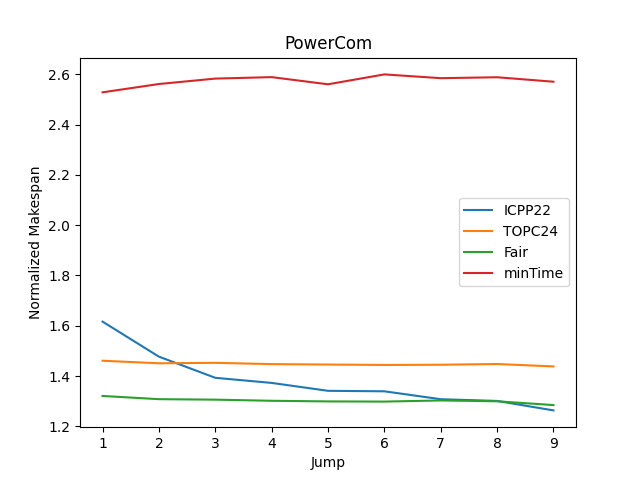
\includegraphics[width=\textwidth]{Results/Jump/Jump_PowerCom}\caption{PowerCom}\label{fig:lines_figures_Jump_PowerCom}\end{subfigure}
\hfill
\caption{Lines Figure for Jump}
\label{fig:lines_figures_Jump}
\end{figure}




\FloatBarrier 
\subsection{Boxplot Figures}
\begin{figure}[htbp]
\centering
\begin{subfigure}[b]{0.32\textwidth}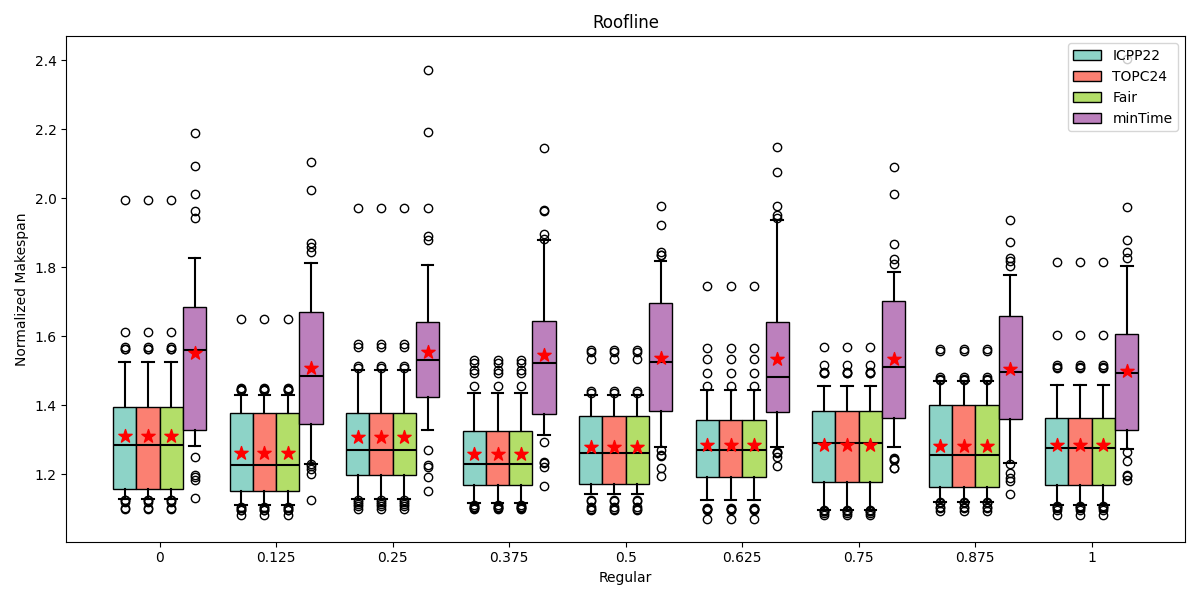
\includegraphics[width=\textwidth]{Results/Regular/Regular_Roofline_boxplot}\caption{Roofline}\label{fig:boxplot_figures_Regular_Roofline}\end{subfigure}
\hfill
\begin{subfigure}[b]{0.32\textwidth}\includegraphics[width=\textwidth]{Results/Regular/Regular_Communication_boxplot}\caption{Communication}\label{fig:boxplot_figures_Regular_Communication}\end{subfigure}
\hfill
\begin{subfigure}[b]{0.32\textwidth}\includegraphics[width=\textwidth]{Results/Regular/Regular_Amdahl_boxplot}\caption{Amdahl}\label{fig:boxplot_figures_Regular_Amdahl}\end{subfigure}
\\[2ex]
\begin{subfigure}[b]{0.32\textwidth}\includegraphics[width=\textwidth]{Results/Regular/Regular_General_boxplot}\caption{General}\label{fig:boxplot_figures_Regular_General}\end{subfigure}
\hfill
\begin{subfigure}[b]{0.32\textwidth}\includegraphics[width=\textwidth]{Results/Regular/Regular_PowerCom_boxplot}\caption{PowerCom}\label{fig:boxplot_figures_Regular_PowerCom}\end{subfigure}
\hfill
\caption{Boxplot Figure for Regular}
\label{fig:boxplot_figures_Regular}
\end{figure}
\begin{figure}[htbp]
\centering
\begin{subfigure}[b]{0.32\textwidth}\includegraphics[width=\textwidth]{Results/Density/Density_Roofline_boxplot}\caption{Roofline}\label{fig:boxplot_figures_Density_Roofline}\end{subfigure}
\hfill
\begin{subfigure}[b]{0.32\textwidth}\includegraphics[width=\textwidth]{Results/Density/Density_Communication_boxplot}\caption{Communication}\label{fig:boxplot_figures_Density_Communication}\end{subfigure}
\hfill
\begin{subfigure}[b]{0.32\textwidth}\includegraphics[width=\textwidth]{Results/Density/Density_Amdahl_boxplot}\caption{Amdahl}\label{fig:boxplot_figures_Density_Amdahl}\end{subfigure}
\\[2ex]
\begin{subfigure}[b]{0.32\textwidth}\includegraphics[width=\textwidth]{Results/Density/Density_General_boxplot}\caption{General}\label{fig:boxplot_figures_Density_General}\end{subfigure}
\hfill
\begin{subfigure}[b]{0.32\textwidth}\includegraphics[width=\textwidth]{Results/Density/Density_PowerCom_boxplot}\caption{PowerCom}\label{fig:boxplot_figures_Density_PowerCom}\end{subfigure}
\hfill
\caption{Boxplot Figure for Density}
\label{fig:boxplot_figures_Density}
\end{figure}
\begin{figure}[htbp]
\centering
\begin{subfigure}[b]{0.32\textwidth}\includegraphics[width=\textwidth]{Results/Fat/Fat_Roofline_boxplot}\caption{Roofline}\label{fig:boxplot_figures_Fat_Roofline}\end{subfigure}
\hfill
\begin{subfigure}[b]{0.32\textwidth}\includegraphics[width=\textwidth]{Results/Fat/Fat_Communication_boxplot}\caption{Communication}\label{fig:boxplot_figures_Fat_Communication}\end{subfigure}
\hfill
\begin{subfigure}[b]{0.32\textwidth}\includegraphics[width=\textwidth]{Results/Fat/Fat_Amdahl_boxplot}\caption{Amdahl}\label{fig:boxplot_figures_Fat_Amdahl}\end{subfigure}
\\[2ex]
\begin{subfigure}[b]{0.32\textwidth}\includegraphics[width=\textwidth]{Results/Fat/Fat_General_boxplot}\caption{General}\label{fig:boxplot_figures_Fat_General}\end{subfigure}
\hfill
\begin{subfigure}[b]{0.32\textwidth}\includegraphics[width=\textwidth]{Results/Fat/Fat_PowerCom_boxplot}\caption{PowerCom}\label{fig:boxplot_figures_Fat_PowerCom}\end{subfigure}
\hfill
\caption{Boxplot Figure for Fat}
\label{fig:boxplot_figures_Fat}
\end{figure}
\begin{figure}[htbp]
\centering
\begin{subfigure}[b]{0.32\textwidth}\includegraphics[width=\textwidth]{Results/n/n_Roofline_boxplot}\caption{Roofline}\label{fig:boxplot_figures_n_Roofline}\end{subfigure}
\hfill
\begin{subfigure}[b]{0.32\textwidth}\includegraphics[width=\textwidth]{Results/n/n_Communication_boxplot}\caption{Communication}\label{fig:boxplot_figures_n_Communication}\end{subfigure}
\hfill
\begin{subfigure}[b]{0.32\textwidth}\includegraphics[width=\textwidth]{Results/n/n_Amdahl_boxplot}\caption{Amdahl}\label{fig:boxplot_figures_n_Amdahl}\end{subfigure}
\\[2ex]
\begin{subfigure}[b]{0.32\textwidth}\includegraphics[width=\textwidth]{Results/n/n_General_boxplot}\caption{General}\label{fig:boxplot_figures_n_General}\end{subfigure}
\hfill
\begin{subfigure}[b]{0.32\textwidth}\includegraphics[width=\textwidth]{Results/n/n_PowerCom_boxplot}\caption{PowerCom}\label{fig:boxplot_figures_n_PowerCom}\end{subfigure}
\hfill
\caption{Boxplot Figure for n}
\label{fig:boxplot_figures_n}
\end{figure}
\begin{figure}[htbp]
\centering
\begin{subfigure}[b]{0.32\textwidth}\includegraphics[width=\textwidth]{Results/P/P_Roofline_boxplot}\caption{Roofline}\label{fig:boxplot_figures_P_Roofline}\end{subfigure}
\hfill
\begin{subfigure}[b]{0.32\textwidth}\includegraphics[width=\textwidth]{Results/P/P_Communication_boxplot}\caption{Communication}\label{fig:boxplot_figures_P_Communication}\end{subfigure}
\hfill
\begin{subfigure}[b]{0.32\textwidth}\includegraphics[width=\textwidth]{Results/P/P_Amdahl_boxplot}\caption{Amdahl}\label{fig:boxplot_figures_P_Amdahl}\end{subfigure}
\\[2ex]
\begin{subfigure}[b]{0.32\textwidth}\includegraphics[width=\textwidth]{Results/P/P_General_boxplot}\caption{General}\label{fig:boxplot_figures_P_General}\end{subfigure}
\hfill
\begin{subfigure}[b]{0.32\textwidth}\includegraphics[width=\textwidth]{Results/P/P_PowerCom_boxplot}\caption{PowerCom}\label{fig:boxplot_figures_P_PowerCom}\end{subfigure}
\hfill
\caption{Boxplot Figure for P}
\label{fig:boxplot_figures_P}
\end{figure}
\begin{figure}[htbp]
\centering
\begin{subfigure}[b]{0.32\textwidth}\includegraphics[width=\textwidth]{Results/Priority/Priority_Roofline_boxplot}\caption{Roofline}\label{fig:boxplot_figures_Priority_Roofline}\end{subfigure}
\hfill
\begin{subfigure}[b]{0.32\textwidth}\includegraphics[width=\textwidth]{Results/Priority/Priority_Communication_boxplot}\caption{Communication}\label{fig:boxplot_figures_Priority_Communication}\end{subfigure}
\hfill
\begin{subfigure}[b]{0.32\textwidth}\includegraphics[width=\textwidth]{Results/Priority/Priority_Amdahl_boxplot}\caption{Amdahl}\label{fig:boxplot_figures_Priority_Amdahl}\end{subfigure}
\\[2ex]
\begin{subfigure}[b]{0.32\textwidth}\includegraphics[width=\textwidth]{Results/Priority/Priority_General_boxplot}\caption{General}\label{fig:boxplot_figures_Priority_General}\end{subfigure}
\hfill
\begin{subfigure}[b]{0.32\textwidth}\includegraphics[width=\textwidth]{Results/Priority/Priority_PowerCom_boxplot}\caption{PowerCom}\label{fig:boxplot_figures_Priority_PowerCom}\end{subfigure}
\hfill
\caption{Boxplot Figure for Priority}
\label{fig:boxplot_figures_Priority}
\end{figure}
\begin{figure}[htbp]
\centering
\begin{subfigure}[b]{0.32\textwidth}\includegraphics[width=\textwidth]{Results/Jump/Jump_Roofline_boxplot}\caption{Roofline}\label{fig:boxplot_figures_Jump_Roofline}\end{subfigure}
\hfill
\begin{subfigure}[b]{0.32\textwidth}\includegraphics[width=\textwidth]{Results/Jump/Jump_Communication_boxplot}\caption{Communication}\label{fig:boxplot_figures_Jump_Communication}\end{subfigure}
\hfill
\begin{subfigure}[b]{0.32\textwidth}\includegraphics[width=\textwidth]{Results/Jump/Jump_Amdahl_boxplot}\caption{Amdahl}\label{fig:boxplot_figures_Jump_Amdahl}\end{subfigure}
\\[2ex]
\begin{subfigure}[b]{0.32\textwidth}\includegraphics[width=\textwidth]{Results/Jump/Jump_General_boxplot}\caption{General}\label{fig:boxplot_figures_Jump_General}\end{subfigure}
\hfill
\begin{subfigure}[b]{0.32\textwidth}\includegraphics[width=\textwidth]{Results/Jump/Jump_PowerCom_boxplot}\caption{PowerCom}\label{fig:boxplot_figures_Jump_PowerCom}\end{subfigure}
\hfill
\caption{Boxplot Figure for Jump}
\label{fig:boxplot_figures_Jump}
\end{figure}


\FloatBarrier 

\subsection{Average Values}
\begin{table}[htbp]
\centering
\caption{Average Values for Each Model and Heuristic}
\label{tab:average_values}
\begin{tabular}{lrrrrr}
\toprule
Model & ICPP22 & TOPC24 & Fair & minTime & minArea \\
Roofline & 1.28 & 1.28 & 1.28 & 1.52 & 11.28 \\
Communication & 1.75 & 1.38 & 1.38 & 2.97 & 10.22 \\
Amdahl & 2.32 & 1.98 & 2.01 & 21.31 & 7.88 \\
General & 2.74 & 1.50 & 1.60 & 4.86 & 5.37 \\
PowerCom & 1.52 & 1.46 & 1.35 & 2.84 & 12.76 \\
\midrule
Average & 1.92 & 1.52 & 1.52 & 6.70 & 9.50 \\
\bottomrule
\end{tabular}
\end{table}

\subsection{Maximum Values}
\begin{table}[htbp]
\centering
\caption{Maximum Values for Each Model and Heuristic}
\label{tab:maximum_values}
\begin{tabular}{lrrrrr}
\toprule
Model & ICPP22 & TOPC24 & Fair & minTime & minArea \\
Roofline & 2.56 & 2.56 & 2.56 & 3.18 & 117.75 \\
Communication & 2.22 & 2.17 & 2.30 & 8.45 & 34.30 \\
Amdahl & 4.52 & 3.75 & 3.76 & 33.26 & 23.45 \\
General & 5.11 & 2.64 & 2.70 & 10.34 & 14.76 \\
PowerCom & 3.71 & 2.16 & 2.46 & 6.83 & 69.98 \\
\midrule
Maximum & 5.11 & 3.75 & 3.76 & 33.26 & 117.75 \\
\bottomrule
\end{tabular}
\end{table}


\FloatBarrier 

\bibliographystyle{plain}
\bibliography{moldable}

\end{document}
